% Document Type and font dimension
\documentclass[12pt]{article}

% Import package to read letters with accents
\usepackage[utf8]{inputenc}

% Import package for font coding
\usepackage[T1]{fontenc}

% Language of the document
\usepackage[english]{babel}

% Set margin
\usepackage[a4paper, margin=1.3in]{geometry}

% Import packages for images
\usepackage{graphicx}
\graphicspath{{img}}
\usepackage[export]{adjustbox}

% Import package for tables
\usepackage{
	tabularborder,
	tabularx,
	multirow,
	multicol,
	longtable}

\title{Eriantys Protocol Documentation}
\author{Giovanni Manfredi, Mattia Martelli, Sebastiano Meneghin\\Group 27}
\date{}

\begin{document}
	
	\maketitle
	
	\section*{Introduction}
	
	The following document will describe the Client-Server communication protocol of the program Eriantys. We used GSON library for serialization and deserialization of messages.
	
	Our group decided to opt for the use of multi threading to manage the variety of different actions the server is required to do. The server is composed of four main threads: \textit{ConnectionHandler, Game, Info and CharacterCard}. This has determined how we explained the protocol in this document: 5 different sequence diagram are present, 4 of which represent separate threads.
	
	Our group decided to focus on the following \textbf{advanced features}:
	%
	\begin{itemize}
		\item Character cards implementation
		\item Four players game
		\item Persistence
	\end{itemize}
	%
	The advanced features that more influenced our communication protocol are the character cards management and saving the game if the connection is lost (persistence). 
	
	\newpage
	
	\section{Messages}
	
		\subsection*{Introduction}
	
		Our group decided to use \emph{parametric messages} for great part of our communication protocol due to the similarities across different messages (in particular the ones regarding in-game communication). \\
		We used five main parametric messages in our protocol, which are: \emph{RequestAction, ResponseAction, RequestValue, ResponseValue, sendInfo}. \\
		\textbf{NB}: these parametric messages are used in the whole program and not only in the section in which they are presented. Tables will be used to simplify the explanation. 
	
	
		\subsection{Connection}
		
			\begin{longtable}{>{\raggedright\arraybackslash}p{0.27\textwidth}|>{\raggedright\arraybackslash}p{0.25\textwidth}|l|>{\raggedright\arraybackslash}p{0.25\textwidth}}
				% First header
				\multicolumn{4}{l}{\textbf{Connection}} \\
				\toprule
				\textbf{MessageName} & \textbf{Description} & \textbf{Sender} & \textbf{Arguments} \\
				\toprule
				\endfirsthead
				% Normal header
				\multicolumn{4}{r}{\footnotesize\itshape Continues from the previous page} \\
				\toprule
				\textbf{MessageName} & \textbf{Description} & \textbf{Sender} & \textbf{Arguments} \\
				\toprule
				\endhead
				% Normal foot
				\midrule
				\multicolumn{4}{r}{\footnotesize\itshape Continues in the next page} \\
				\endfoot
				% Final foot
				\bottomrule
				\endlastfoot
		
				% First page of the table
				registerNewPlayer & Sends information required to connect to the server and to be identified as a player. & 
				Client & \emph{String} username: username of the player. \newline
				\emph{Int} magicAge: for how may years has the player known magic.  \\
				\midrule
				requestResumeGame & Asks the player if he wants to resume an interrupted game. & 
				Server & \\
				\midrule
				responseResumeGame & Responds to requestResumeGame received. & 
				Client & \emph{Boolean} resume: true if the player wants to resume a game. \\
				\midrule
				signalWaitConnection Status & Notifies player that he will wait the connection of other players. & 
				Server & \\
				\midrule
				signalGameStart & Notifies player the start of the game & Server. & \\
				
				% Second page of the table
				requestRules & Requests player a new set of rule he desires to play with. &
				Server & \\
				\midrule
				responseRules & Responds to responseRules with a new set of rules. & 
				Client & \emph{Int} numOfPlayers: number of players that will participate in a game. \newline
				\emph{Boolean} expertRule: true if the player wants to play a game in expertMode. \\
				\midrule
				requestWizard & Asks the player which Wizard Deck he wants to play with. & 
				Server & \emph{Wizard[]} availableWizards: a wizard deck with the cards that haven’t been selected by other players. \\
				\midrule
				responseWizard & Responds to requestWizard. &
				Client & \emph{Wizard} selectedWizard: wizard selected by the player from available wizards. \\
				\midrule
				signalPlayer Disconnected & Notifies to the players that they will be disconnected since one player left the game and disconnects them. &
				Server & \\
				\midrule
				signalGameInProgress & Notifies to the player that a game is already ongoing and disconnects him. &
				Server & \\
			\end{longtable}
	
			\newpage
	
		\subsection{Game}
	
			\begin{longtable}{>{\raggedright\arraybackslash}p{0.27\textwidth}|>{\raggedright\arraybackslash}p{0.25\textwidth}|l|>{\raggedright\arraybackslash}p{0.25\textwidth}}
				% First header
				\multicolumn{4}{l}{\textbf{Game}} \\
				\toprule
				\textbf{MessageName} & \textbf{Description} & \textbf{Sender} & \textbf{Arguments} \\
				\toprule
				\endfirsthead
				% Normal header
				\multicolumn{4}{r}{\footnotesize\itshape Continues from the previous page} \\
				\toprule
				\textbf{MessageName} & \textbf{Description} & \textbf{Sender} & \textbf{Arguments} \\
				\toprule
				\endhead
				% Normal foot
				\midrule
				\multicolumn{4}{r}{\footnotesize\itshape Continues in the next page} \\
				\endfoot
				% Final foot
				\bottomrule
				\endlastfoot
			
				% First page of the table
				requestValue & Asks for the value of a generic field. \textbf{Parametric message}. &
				Client & \emph{String} fieldName: name of the field is requested the value of. \\
				\midrule
				responseValue & Responds to requestValue with the value of the field requested. \textbf{Parametric message}.&
				Server & \emph{<type> fieldValue:} value of the field. \newline i.e.\ type = int[], Color[], \ldots \\
				\midrule
				sendInfo & Sends all the information about the GameBoard (after the setUpPhase) or its changes any time its modified. \textbf{Parametric message}. &
				Server & \emph{Int} numOfFields: number of the field/fieldArray included in the message. \newline
								\emph{<type>} fieldArray[]: various fields are needed to update local player data, \newline 
								i.e.\ professorsLocation, emptiedCloudTile \\
				\midrule
				signalWaitTurnStatus & Notifies player that he has to wait another player turn. &
				Server & \\
				\midrule
				signalGameTurn
				Status & Notifies player that has started his turn. &
				Server & \\
			
				% Second page of the table
				requestAction & Requests player to make an action (i.e choose an assistantCard, move students) between provided options. \textbf{Parametric message}. &
				Server & \emph{<type>} fieldArray[]: options for a specific field to choose from, \newline i.e.\ studentsArray, fillCloudTileArray \\
				\midrule
				responseAction & Responds to requestAction with the option selected by the player. \textbf{Parametric message}. &
				Client & \emph{<type>} field: value selected by the player \\
			\end{longtable}
			
			\newpage
			
		\subsection{EndGame}
		
			\begin{longtable}{>{\raggedright\arraybackslash}p{0.27\textwidth}|>{\raggedright\arraybackslash}p{0.25\textwidth}|l|>{\raggedright\arraybackslash}p{0.25\textwidth}}
				% First header
				\multicolumn{4}{l}{\textbf{EndGame}} \\
				\toprule
				\textbf{MessageName} & \textbf{Description} & \textbf{Sender} & \textbf{Arguments} \\
				\toprule
				\endfirsthead
				% Normal header
				\multicolumn{4}{r}{\footnotesize\itshape Continues from the previous page} \\
				\toprule
				\textbf{MessageName} & \textbf{Description} & \textbf{Sender} & \textbf{Arguments} \\
				\toprule
				\endhead
				% Normal foot
				\midrule
				\multicolumn{4}{r}{\footnotesize\itshape Continues in the next page} \\
				\endfoot
				% Final foot
				\bottomrule
				\endlastfoot
			
				% First page of the table
				signalGameResult & Updates player about the end of the match and the winner(s) (including draws). & 
				Server & \emph{GameResult<enum>} gameResult: value indicating the result of the game, depending on how game has finished. \\
				\midrule
				requestReMatch & Asks to the player if he wants to play another game with same players and same rules. &
				Server & \\
				\midrule
				responseReMatch & Responds to requestReMatch. &
				Client & \emph{Boolean} rematch: true if the player wants to play another game. \\
				\midrule
				signalEndGame & Updates player about other players choice about a re-match and disconnect him. &
				Server & \\			
			\end{longtable}
	
			\newpage
			
	\section{Scenarios}
	
		\subsection*{Introduction}
		As previously mentioned we divided the program into five sections. For each one of them we created a sequence diagram showing the different messages of the protocol we just explained above. In this documentation we will analyze the different sections in details, so it has been necessary to crop the original sequence diagrams. The unaltered versions are presented at the end of their respective sections. 
	
		\subsection{Connection}
		
			\subsubsection{Connecting to the server}
			
				\begin{center}
					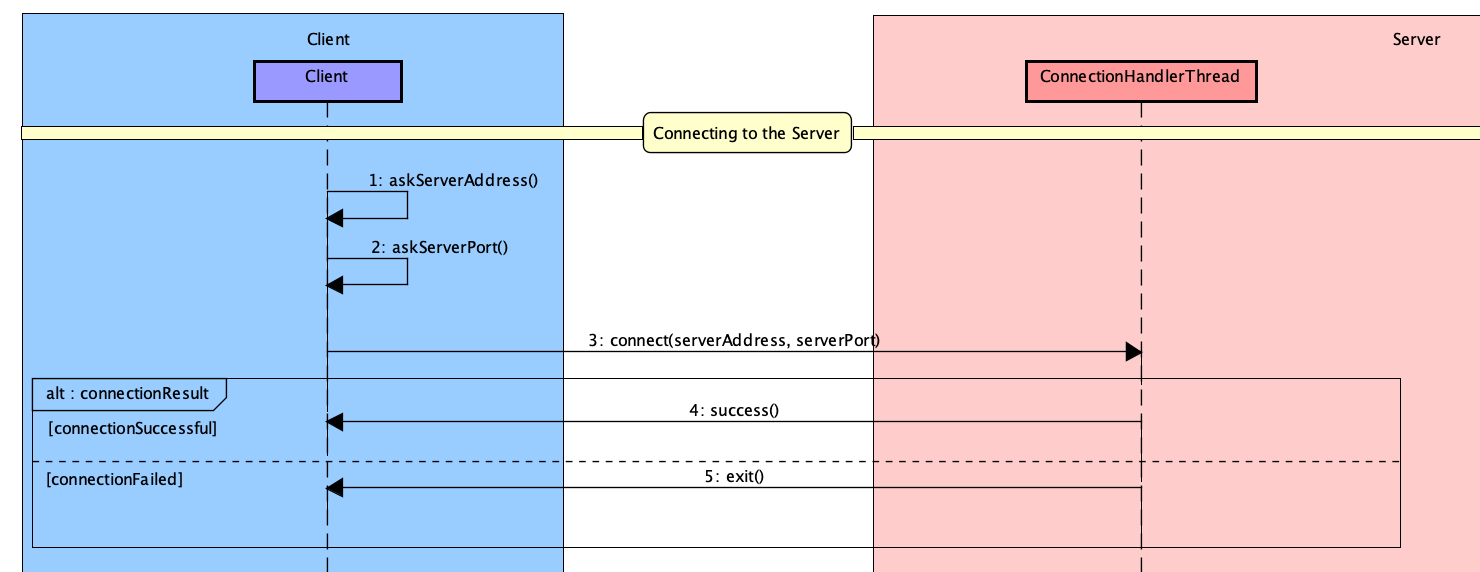
\includegraphics[width=\textwidth,height=\textheight,keepaspectratio]{Connection_1}
				\end{center}
			
				First, the client is asked internally for the ServerAddress and the ServerPort he wants to connect to. Then the client sends this information in the message \emph{connect(serverAddress, serverPort)}. If the server responds with \emph{success()}, the connection is ready to receive the registration related messages. \\
				\textbf{NB}: The server handles the connection with a dedicated thread: \textbf{ConnectionHandler}.
				
			\subsubsection{Registering a player}
			
				\begin{center}
					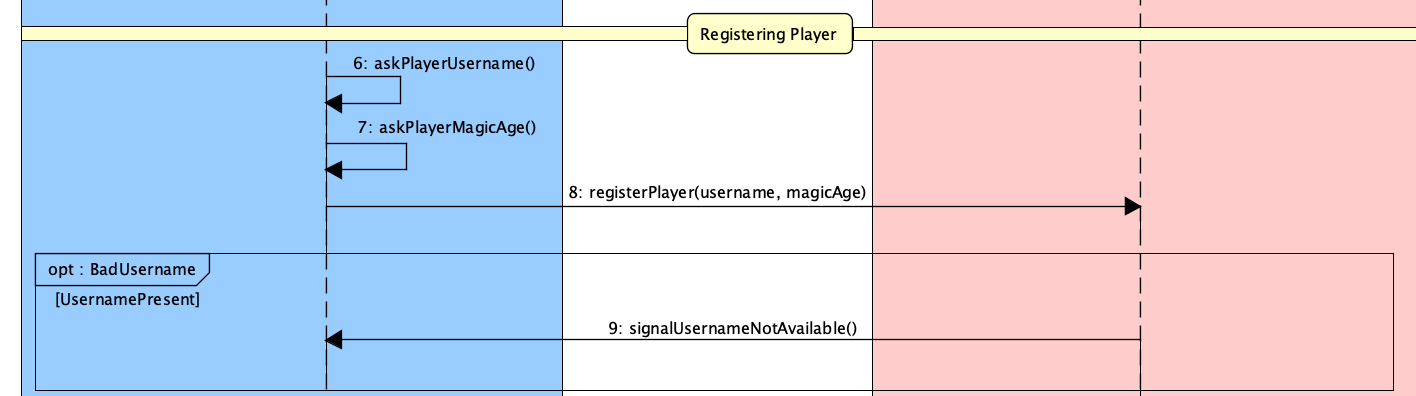
\includegraphics[width=\textwidth,height=\textheight,keepaspectratio]{Connection_2}
				\end{center}
			
				The client is asked internally for his username and magicAge (for how many years has he known magic). Then the client sends this information in the message \emph{registerPlayer(username, magicAge)}. If the server responds with \emph{signalUsernameNotAvailable}, another player with the same username is already connected to the server so the client is disconnected with a message explaining the issue.
				
			\subsubsection{Creating a new game}
			
				\begin{center}
					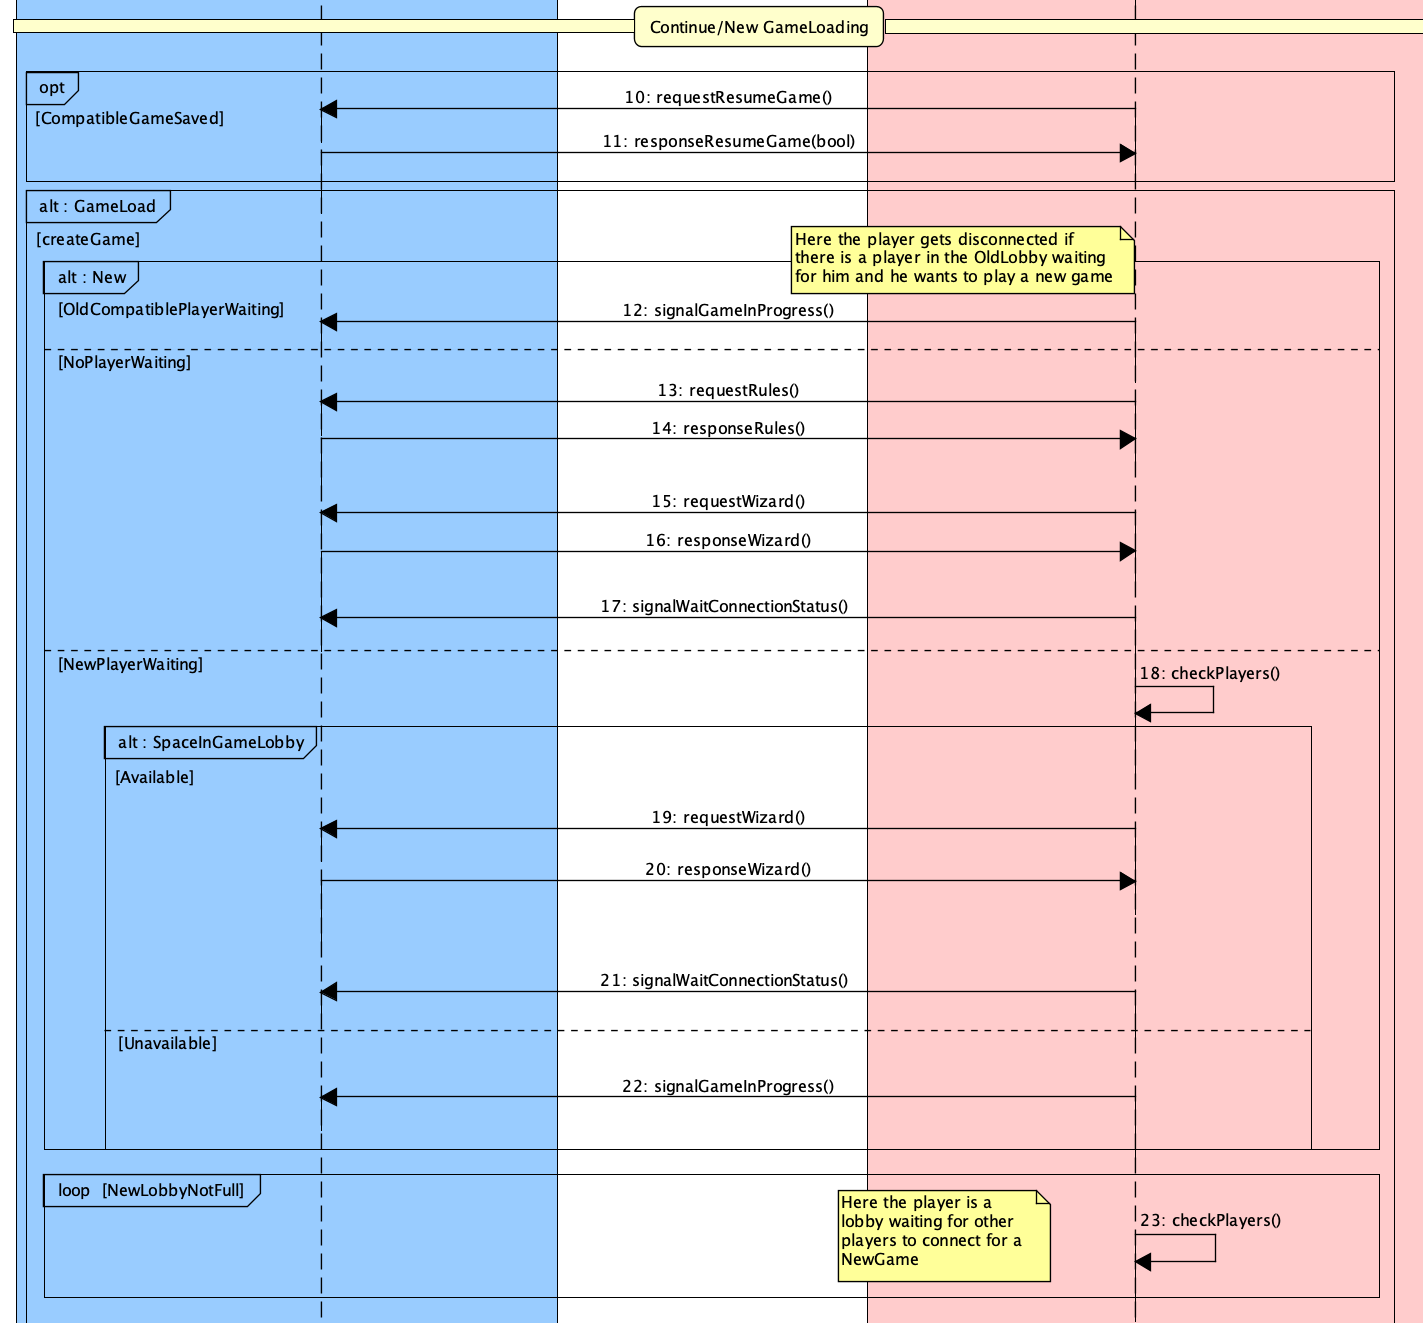
\includegraphics[width=\textwidth,height=\textheight,keepaspectratio]{Connection_3}
				\end{center}
			
				The server sends the client a \emph{requestResumeGame()} if a saved game is present in the server with a username equal to the client's. The client, if it has received this message, responds with \emph{responseResumeGame(bool)} indicating the choice to resume his game (1 \(\rightarrow\) true, 0 \(\rightarrow\) false). \\
				If the client didn't receive \emph{requestResumeGame()} or chose to not resume his old game the alternative taken by the program is [createGame]. \\
				Then based on the other players already connected to the server there could be three different scenarios:
				%
				\begin{itemize}
					\item  \textbf{OldCompatiblePlayerWaiting}: one or more players compatible with a saved game are currently waiting in the OldLobby. The client gets disconnected when he receives \emph{signalGameInProgress()} explaining the issue.
					\item  \textbf{NoPlayerWaiting}: no player is currently waiting for a game, so the server sends \emph{requestRules()} and \emph{requestWizard()} which ask the rules for the new game and which wizard (nature, desert, cloud or snow) the client wants to play with respectively. The client responds with \emph{responseRules()} and \emph{responseWizard()} indicating which rules (int numberOfPlayers, bool expertMode) and which wizard (enum chosenWizard) he wants to play with. \\
					\textbf{NB}: The first player who connects to the newLobby is the one who decides the rules of the game, the other players connect to his lobby if space is still available.
					\item  \textbf{NewPlayerWaiting}: a player is currently waiting for a new game (in the NewLobby) so we check if there is still space available in the lobby. If there is still space the servers asks the player which wizard he wants to play with through the request-response: \emph{requestWizard(), responseWizard()}. Then the server informs the player using the message \emph{signalWaitConnectionStatus()} that he is in the lobby waiting for new players to connect and start the game.
				\end{itemize}
				%
				Finally the server waits for new players to connect checking in a loop if the NewLobby is full. Once the lobby is full the server is ready to create a new game.
								
			\subsubsection{Resuming an old game}
			
				\begin{center}
					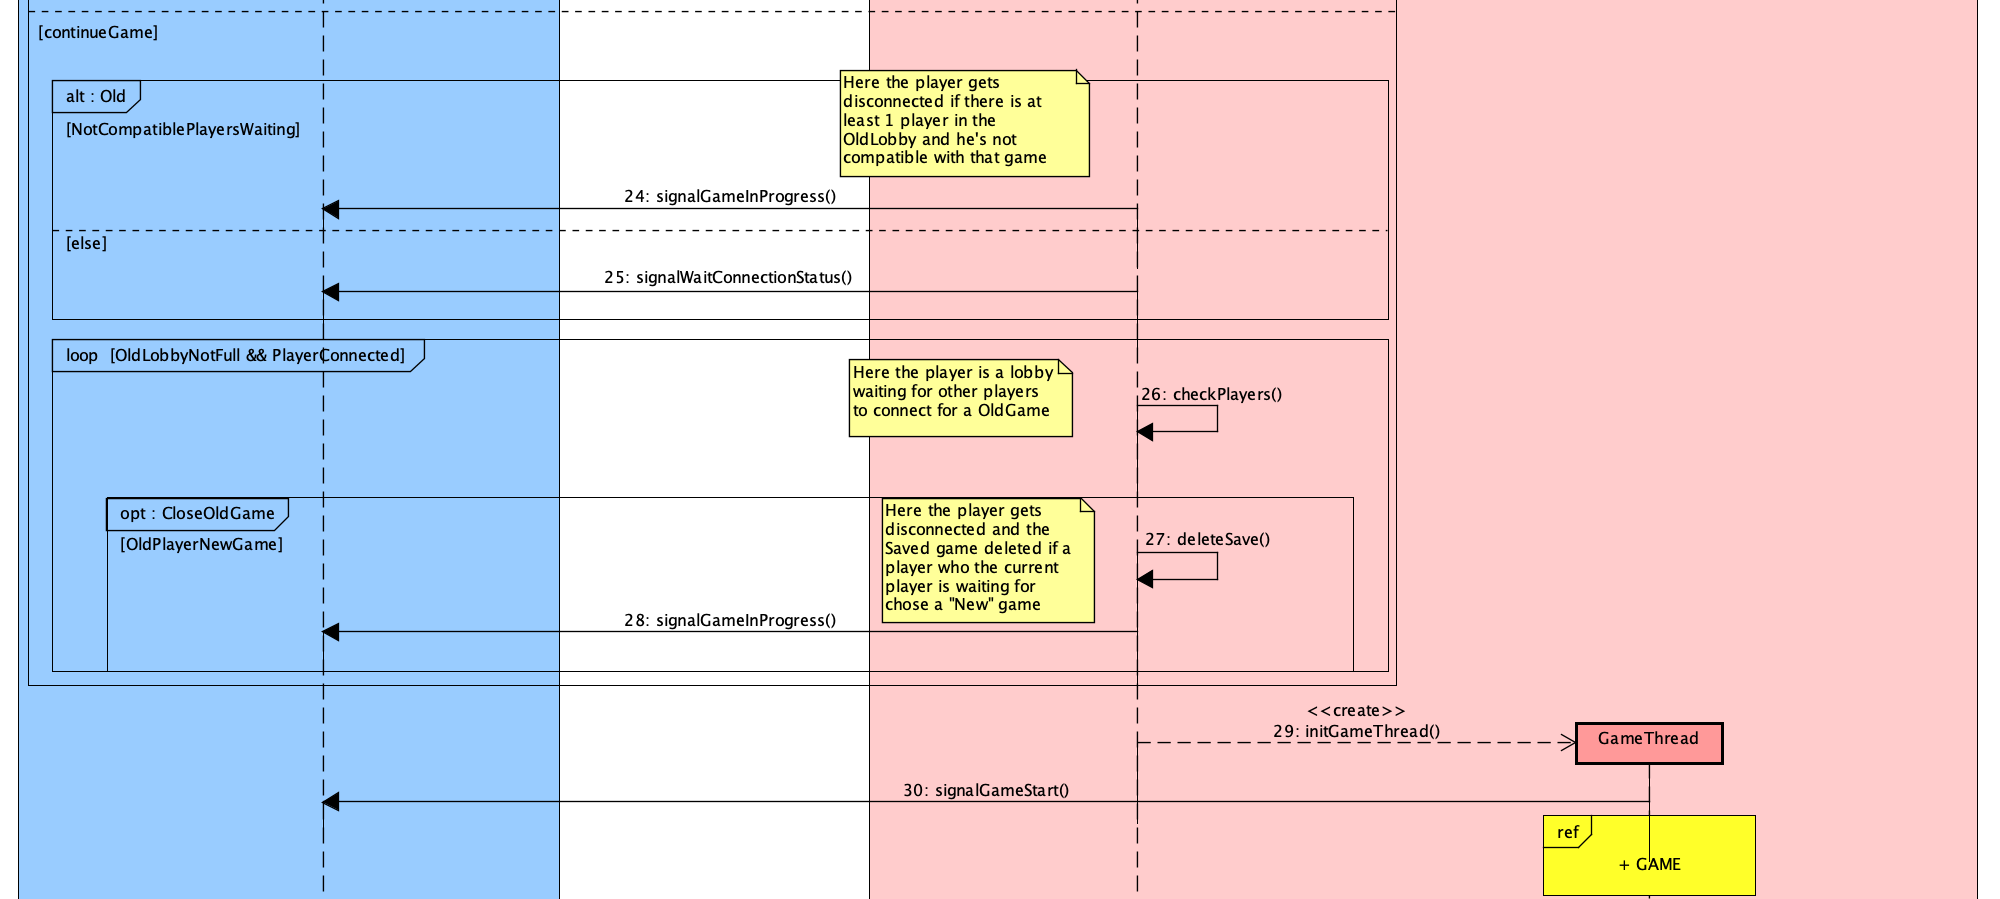
\includegraphics[width=\textwidth,height=\textheight,keepaspectratio]{Connection_4}
				\end{center}
			
				If the player received \emph{requestResumeGame()} and chose to resume his old game the alternative taken by the program is [resumeGame]. \\
				Then based on the other players already connected to the server there could be two different scenarios:
				%
				\begin{itemize}
					\item \textbf{NotCompatiblePlayersWaiting}: one or more players are waiting for a game not compatible with the client (OldNotCompatible game or NewGame). The client gets disconnected when he receives \emph{signalGameInProgress()} explaining the issue.
					\item \textbf{CompatiblePlayersWaiting or NoPlayerWaiting}: alternatively the player receives \emph{signalWaitConnectionStatus()} informing him that he is connected to the OldLobby waiting for the oldPlayer to join.
				\end{itemize}
				%
				Finally the servers waits for the old compatible players to connect checking in a loop if the OldLobby is full. If a player the server is waiting for to start the game connects but decides to begin a new game, the server deletes the save and informs the other players waiting for him of the issue and disconnects them with \emph{signalGameInProgress()}.
				
				Out of the alternative block called GameLoad, the program now has a full lobby so the ConnectionHandler initializes GameThread that when created informs the client with the message \emph{signalGameStart()}.	
				
				\textbf{NB}: a new game will begin with a SetupPhase and will be followed by the consecutive phases, whereas a resumed game will begin with the saved state and continue the game from there. 			
				
			\subsubsection{Disconnecting during a game}
			
			\begin{center}
				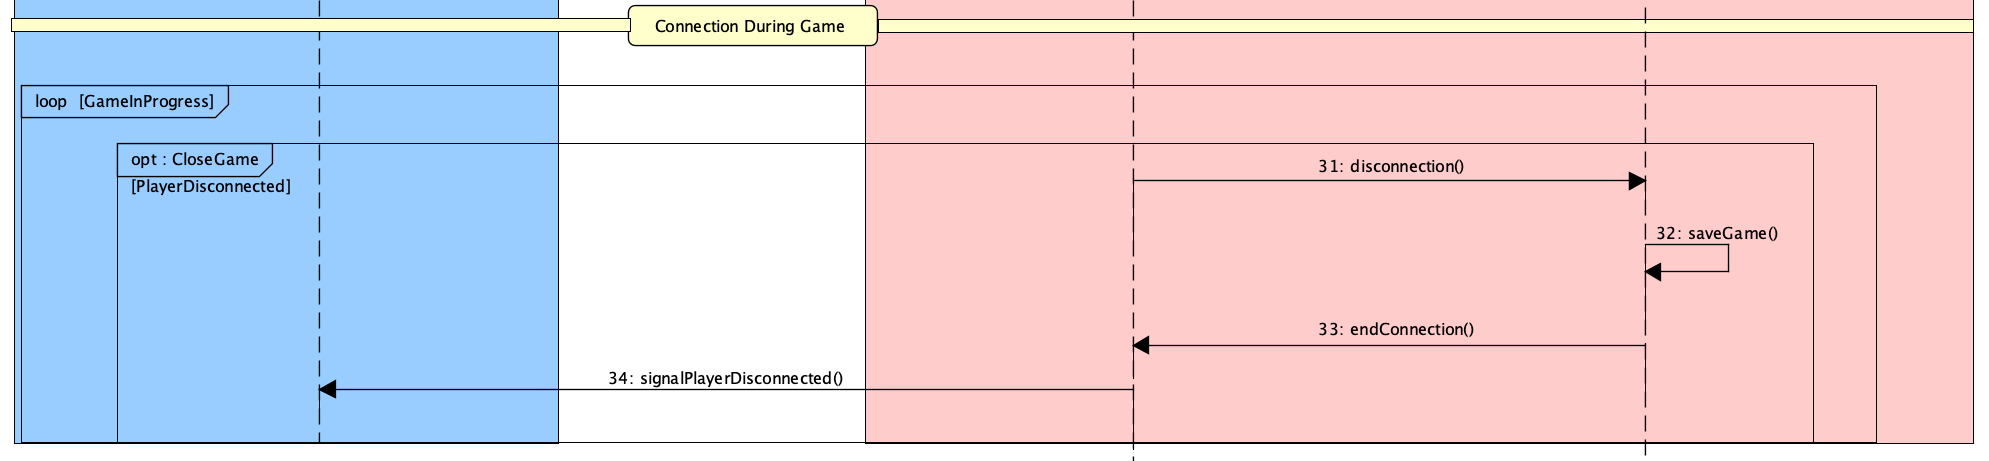
\includegraphics[width=\textwidth,height=\textheight,keepaspectratio]{Connection_5}
			\end{center}
			
			During the game the \textbf{ConnectionHandlerThread} handles the disconnections by the client. The server loops an optional condition of disconnection that if reached informs the GameThread, which saves the game and asks the ConnectionHandler to close the connection. The ConnectionHandler sends \emph{signalPlayerDisconnection()} to inform the client of the issue and to disconnect him.
			
					
		\begin{figure}[htp]
			\centering
			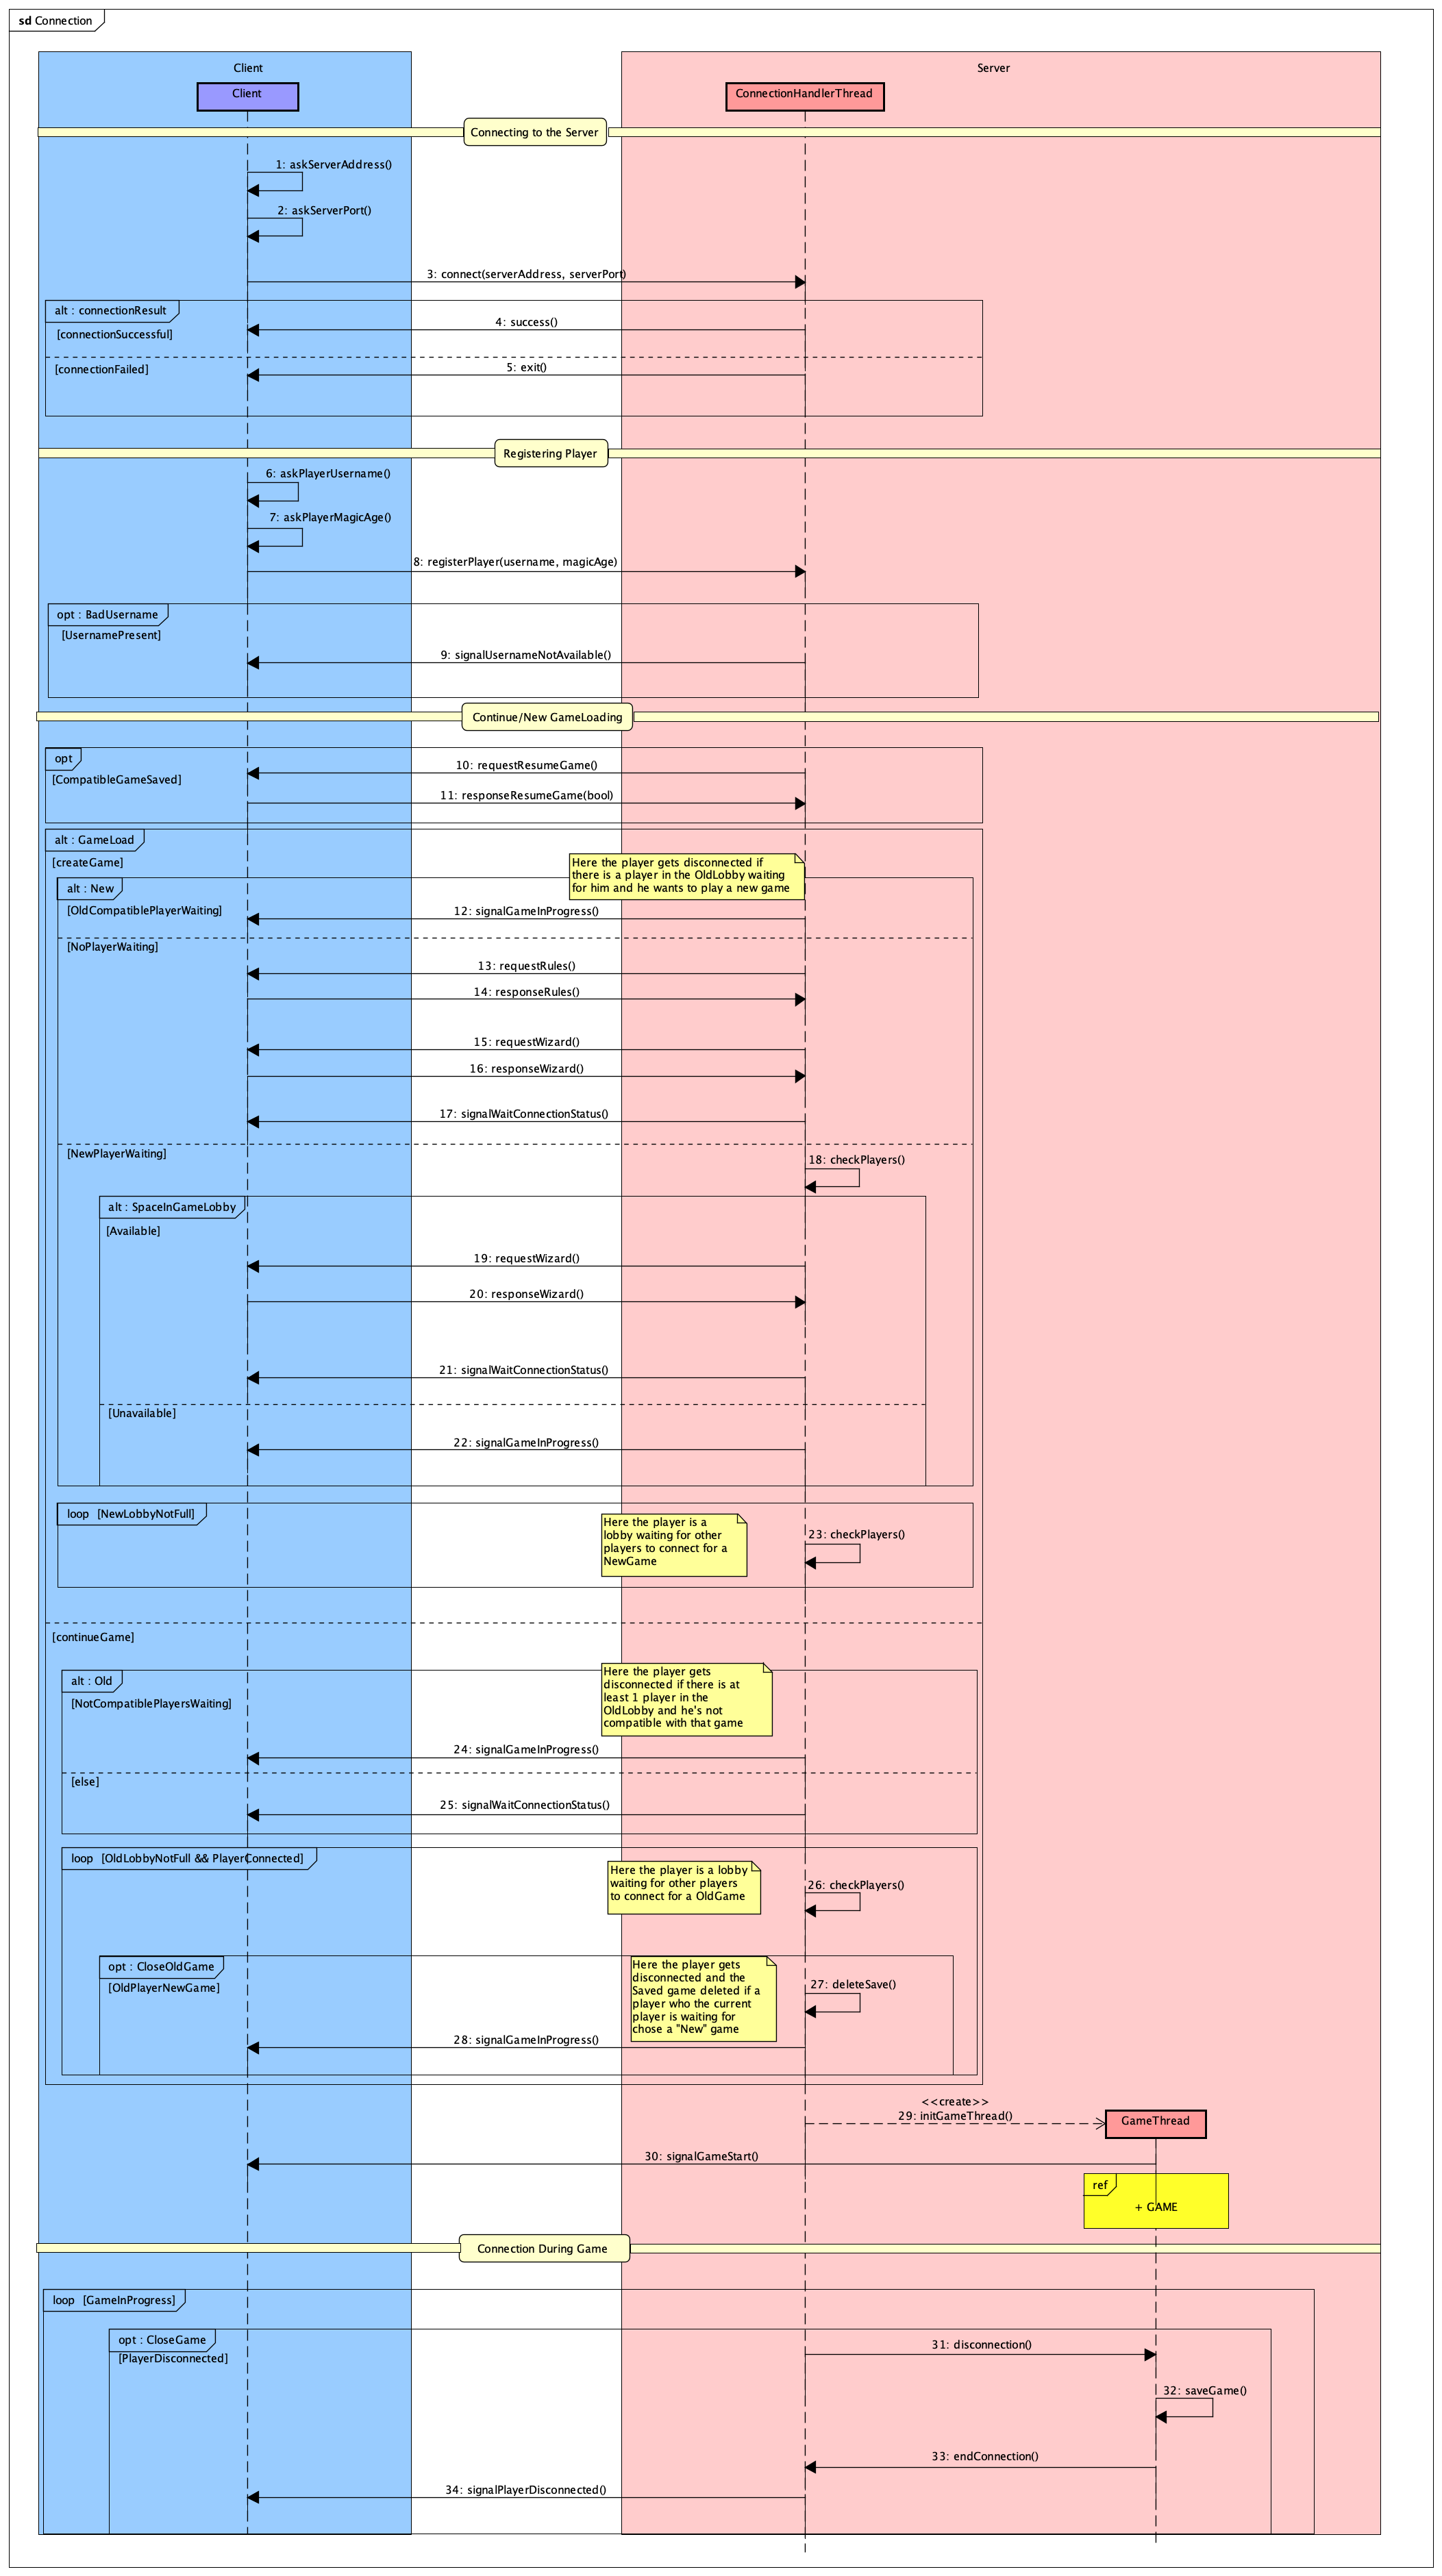
\includegraphics[width=\textwidth,height=\textheight,keepaspectratio]{Connection}
		\end{figure}
	
		\newpage
	
		\subsection{Game}
		
			\subsubsection{SetupPhase and PlanPhase}
				
				\begin{center}
					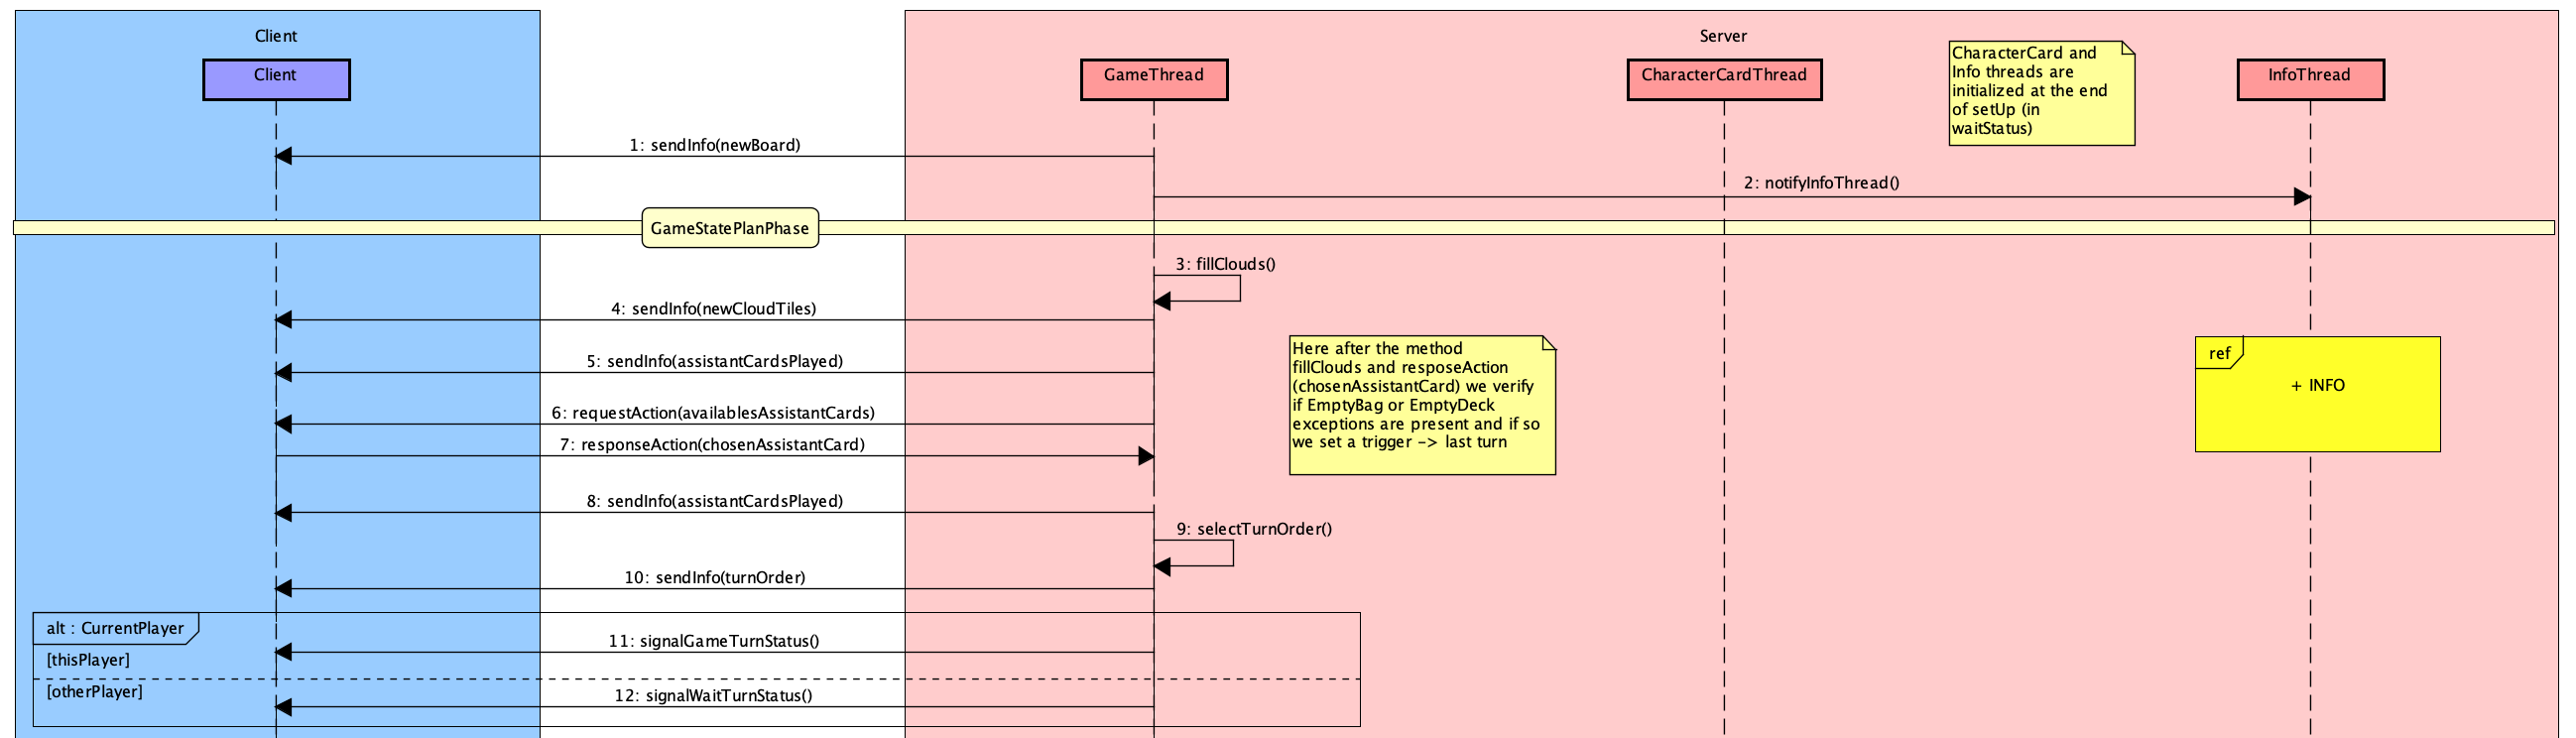
\includegraphics[width=\textwidth,height=\textheight,keepaspectratio]{Game_1}
				\end{center}
				
				The first phase of the game is the Setup, which is not shown in these diagrams because it is mainly composed of methods internal to the server. \\
				At the end of the SetupPhase the server sends the information regarding the game board to the client using a \emph{sendInfo(newBoard)}. GameThread also notifies InfoThread waking him up. After this message InfoThread will be active simultaneously with GameThread, answering requests from the Client for values of the Model.
				
				The server begins the PlanningPhase which is composed of three sections:
				%
				\begin{itemize}
					%
					\item \textbf{FillClouds}: the server fills the CloudTiles with students extracting them from the Bag. If the Bag is empty, it triggers the \emph{EmptyBagException} that will set a trigger which is then checked in the last phase: if the trigger is set this will be the last turn of the game. \\
					The server then informs the players with the message \emph{sendInfo(newCloudTiles)}.
					%
					\item \textbf{PlayAssistantCard}: the server informs the players with what AssistantCards have already been played with \emph{sendInfo(assistantCardsPlayed)} and then asks him what AssistantCard he wants to play from an available pool with \emph{requestAction(availableAssistantCards)}. The client responds with the card he wants to play using the message \emph{responseAction(chosenAssistantCard)}. The server further replies by sending \emph{sendInfo(assistantCardsPlayed)} informing the client and the other players on what AssistantCard was just played. 
					%
					\item \textbf{SelectTurnOrder}: the server selects a turn order based on the played cards and sends the client a \emph{sendInfo(TurnOrder)} to inform him on the turn order. Then the client could be the firstPlayer or not, if he is, the server notifies him with a \emph{signalGameTurnStatus()} indicating that he will now start his turn. Alternatively, the server informs him with \emph{signalWaitTurnStatus()} that he will wait another player's turn. 
					%
				\end{itemize}
				
			\subsubsection{ActionPhase - MoveStudents and CharacterCards}
			
				\begin{center}
					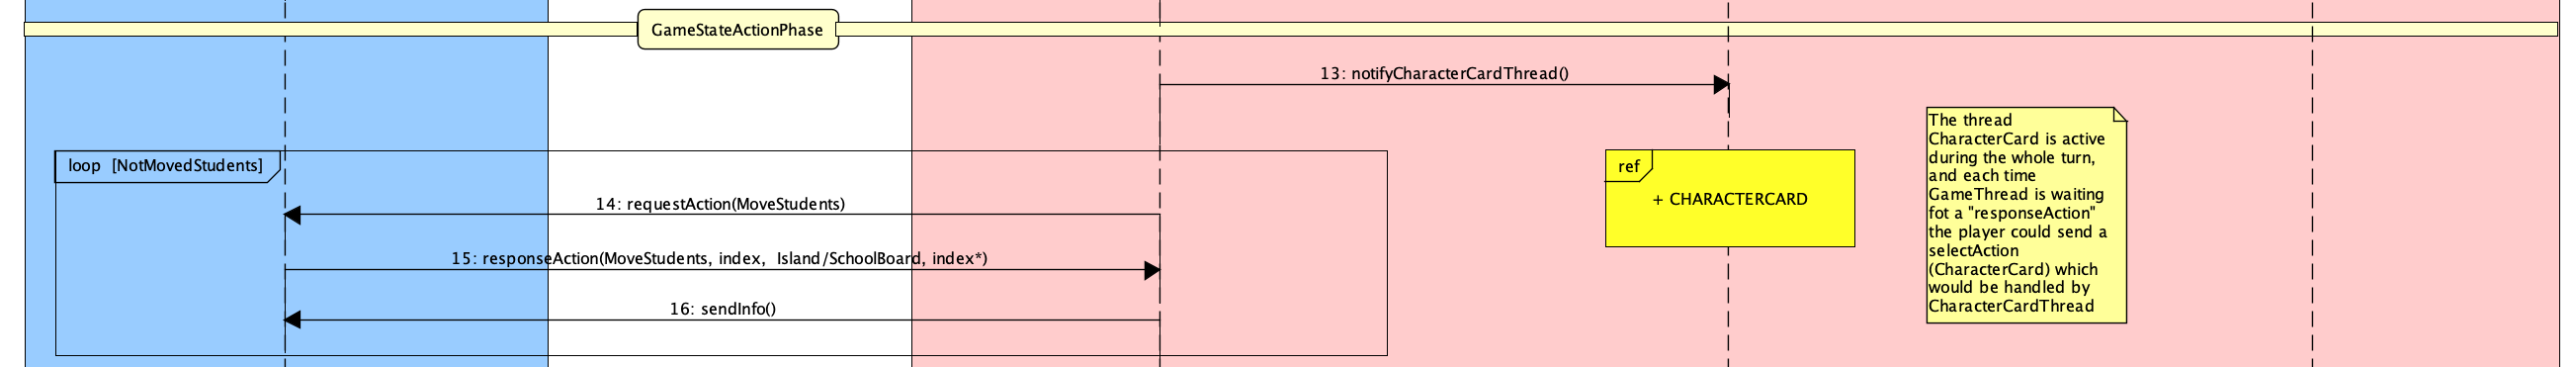
\includegraphics[width=\textwidth,height=\textheight,keepaspectratio]{Game_2}
				\end{center}
				
				At the beginning of the ActionPhase the GameThread notifies CharacterCardThread waking him up: it will be now be possible for the client to send requests to use a CharacterCard. \\
				The server then enters a loop (of three cycles) to allow the client to move his students. GameThread sends a \emph{requestAction(MoveStudents)} to which the client responds with a \emph{responseAction(MoveStudents, index, Island/SchoolBoard, index*)} specifying the student counter the client wants to move and where he wants to move it. After the movement the server updates the client with a \emph{sendInfo()}.
								
			\subsubsection{ActionPhase - MoveMotherNature}
			
				\begin{center}
					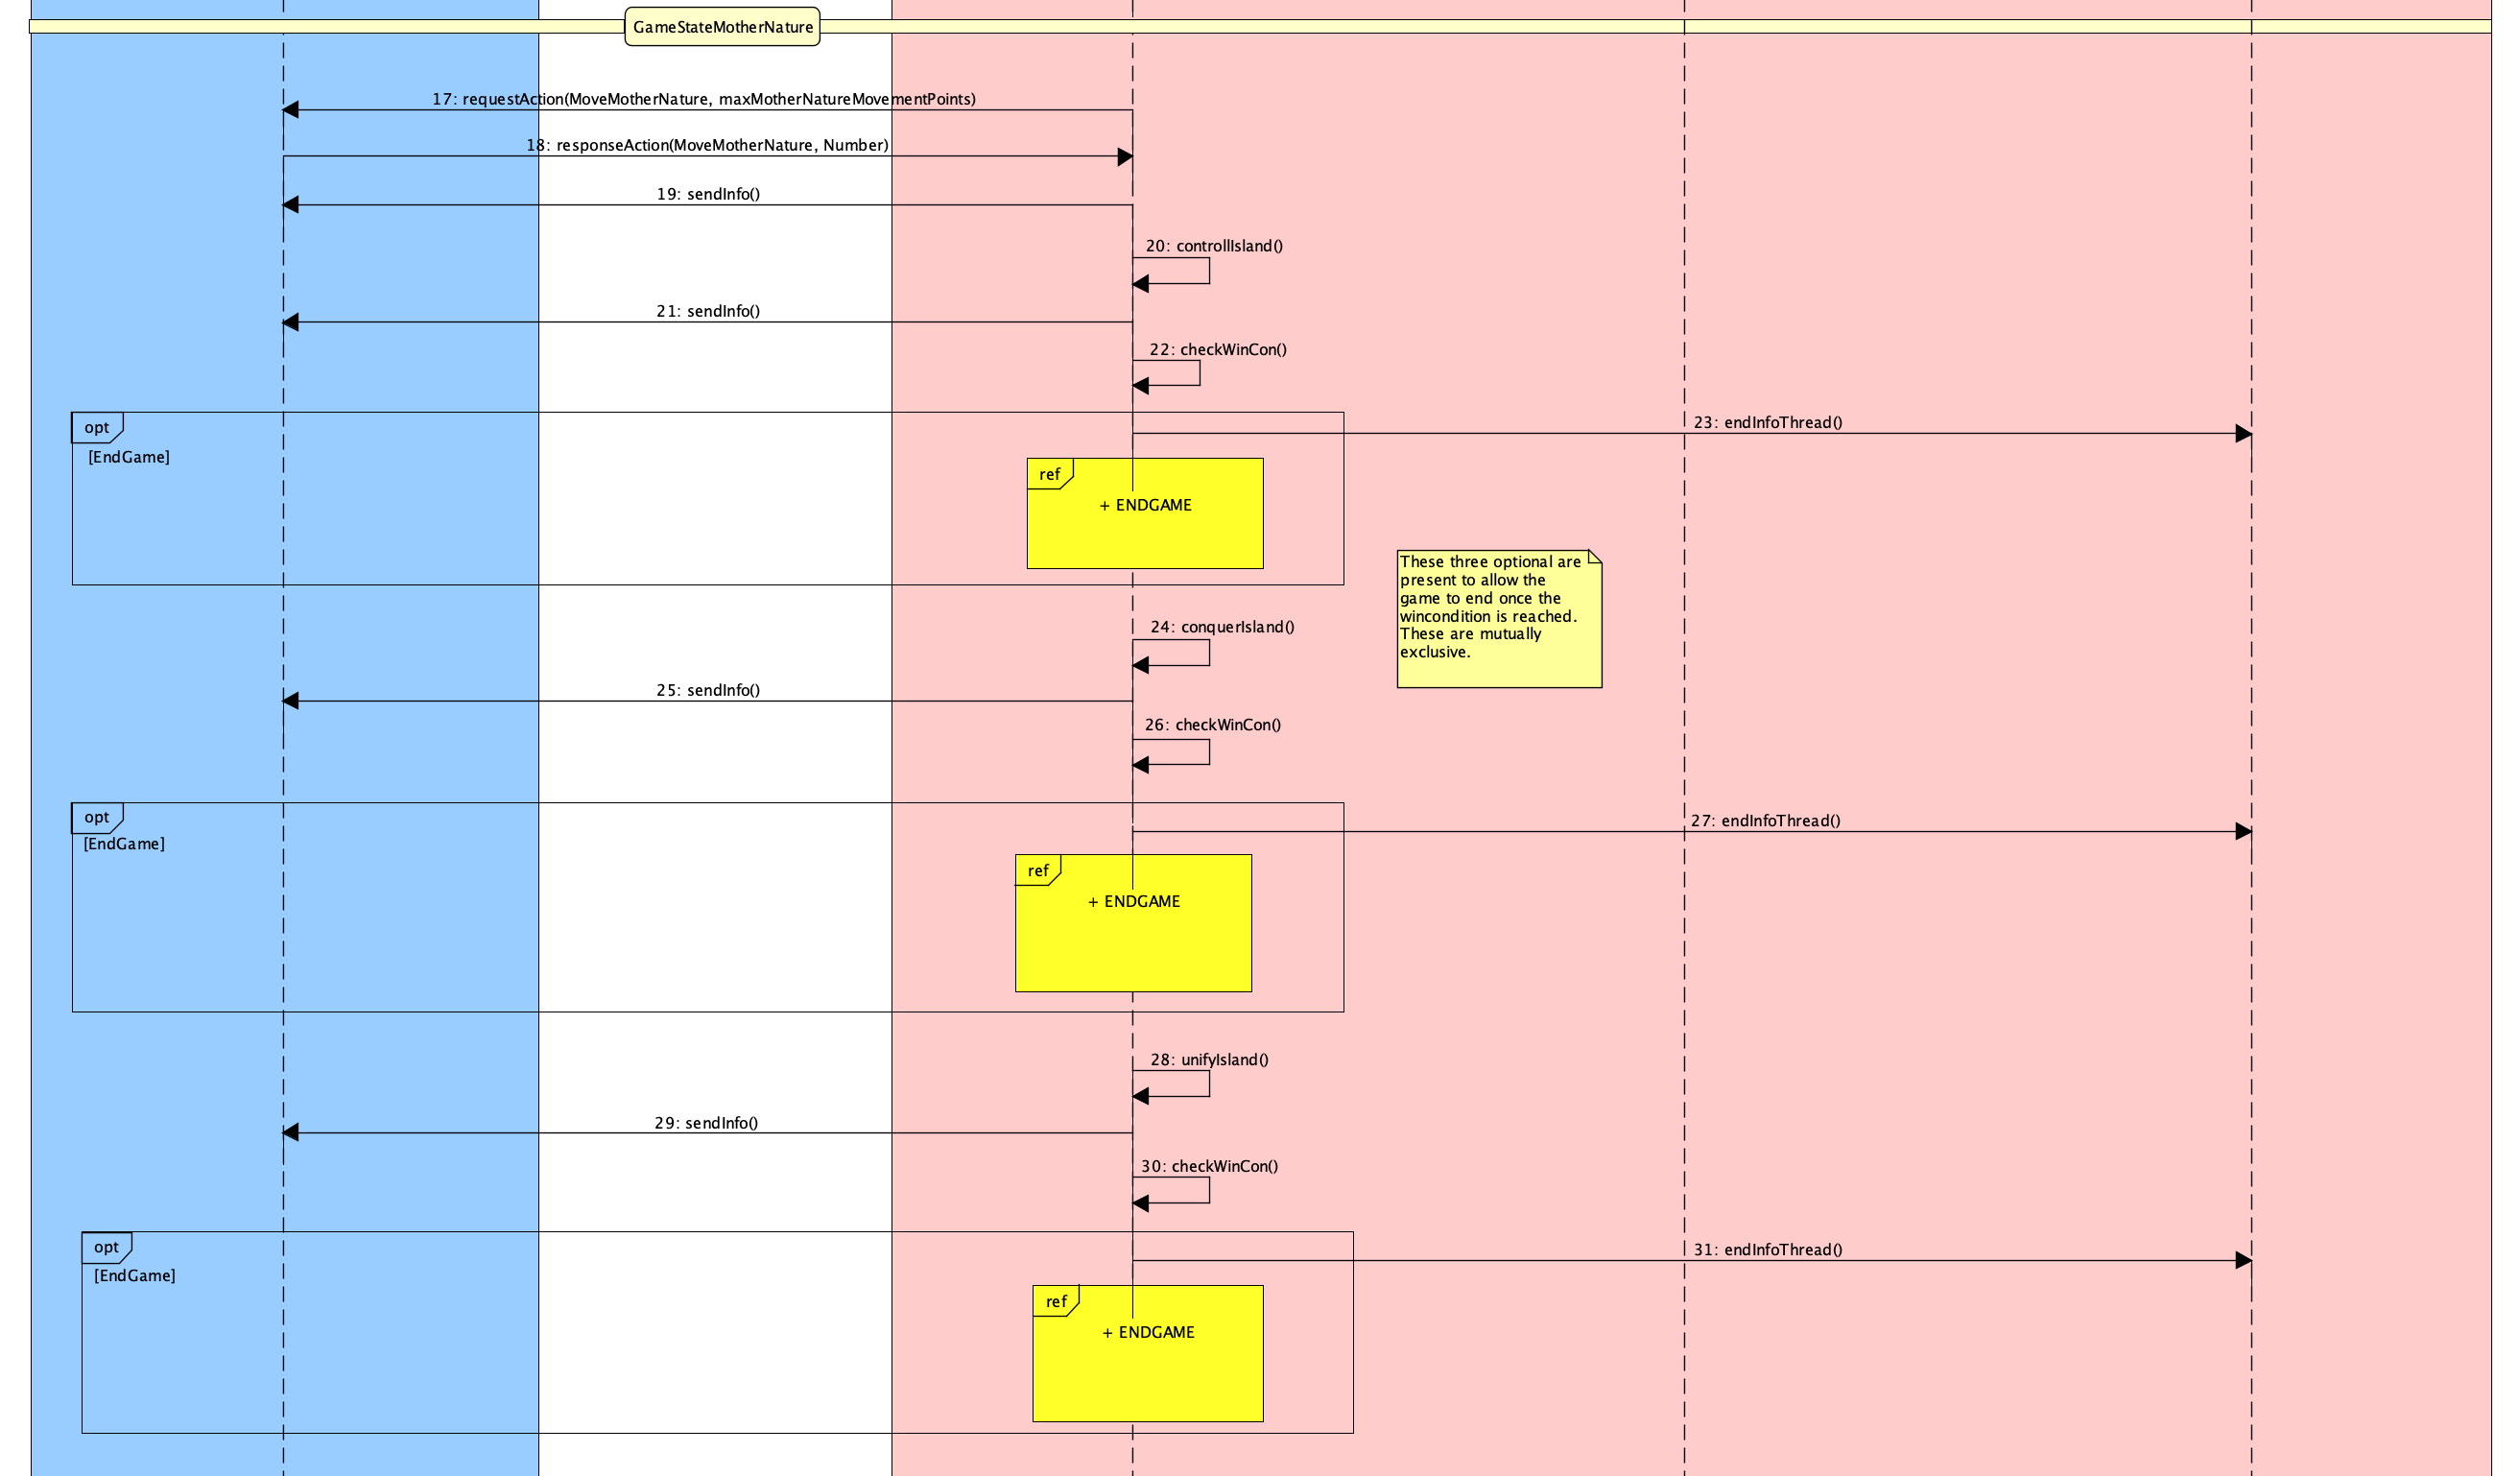
\includegraphics[width=\textwidth,height=\textheight,keepaspectratio]{Game_3}
				\end{center}
				
				First, the GameThread sends a \emph{requestAction(MoveMotherNature, maxMotherNatureMovementPoints)} asking the player to move Mother Nature of a positive value smaller or equal to parameter. The client replies with a \emph{responseAction(MoveMotherNature, number)} specifying where he wants to move Mother Nature. The server then moves it and then informs the players with a \emph{sendInfo()}. \\
				Subsequently GameThread applies the three effects of Mother Nature's movement which are:
				%
				\begin{itemize}
					\item \textbf{ControlIsland}: if no tower is present on the island (on which Mother Nature finished the turn on), the server calculates the influence on the island and places the tower of the player with the highest influence on that island. Then, after informing the client with a \emph{sendInfo()}, the GameThread controls if the winning condition is reached (all towers of a player played), and if so, it enters in a optional block called ``EndGame''.
					\item \textbf{ConquerIsland}: if one or more towers are present on the island the server calculates the influence on the island (on which Mother Nature finished the turn on) and replaces the tower with the one of the player with the highest influence on that island. Then, after informing the client with a \emph{sendInfo()}, the GameThread controls if the winning condition is reached (all towers of a player played), and if so, it enters in a optional block called ``EndGame''.
					\item \textbf{UnifyIsland}: if the adjacent islands (either or both) to the island (on which Mother Nature finished the turn on) have towers of the same TowerColor to the current island, the server unifies the islands (from three to one or from two to one). Then, after informing the client with a \emph{sendInfo()}, the GameThread controls if the winning condition is reached (three or less islands on board), and if so, it enters in a optional block called ``EndGame''. 
				\end{itemize}
				
			\subsubsection{ActionPhase - ChooseCloud}
			
				\begin{center}
					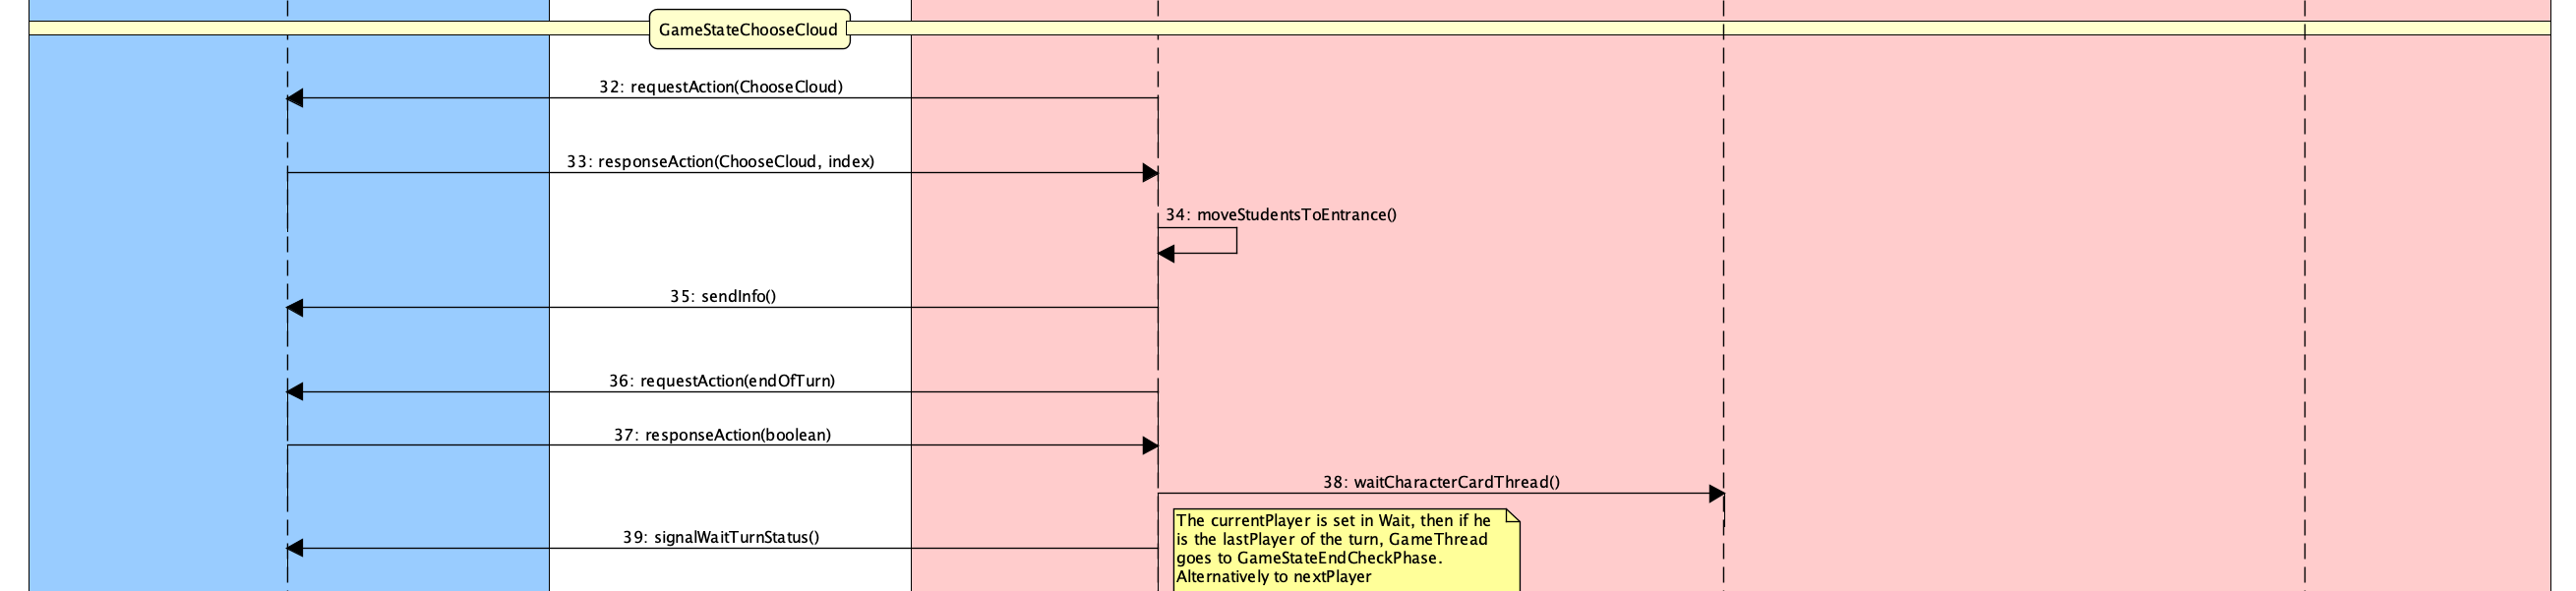
\includegraphics[width=\textwidth,height=\textheight,keepaspectratio]{Game_4}
				\end{center}
				
				First the client is asked which CloudTile he is going to select with the message \emph{requestAction(ChooseCloud)} to which the client responds with \emph{responseAction(ChooseCloud, index)} specifying the CloudTile he chose. Then the GameThread after having moved the students from the chosen CloudTile to the Entrance of the player shows him the updated GameBoard with a \emph{sendInfo()}. \\
				Finally the server asks the client if he wants to end his turn using \emph{requestAction(endOfTurn)} to which the client responds with \emph{responseAction(boolean)} containing his decision (1 \(\rightarrow\) true, 0 \(\rightarrow\) false). The server waits until he receives a positive response (with value 1) and after receiving it, he ends the turn. \\
				CharacterCardThread is informed and set to a waitStatus and the client receives a \emph{signalWaitTurnStatus} which makes him wait for another player to play. 
				After this Phase, GameThread goes to the next player, starting the turn from the ActionPhase, or if the current player was the last player GameThread continues in the EndCheckPhase.
							
			\subsubsection{EndCheckPhase}
			
				\begin{center}
					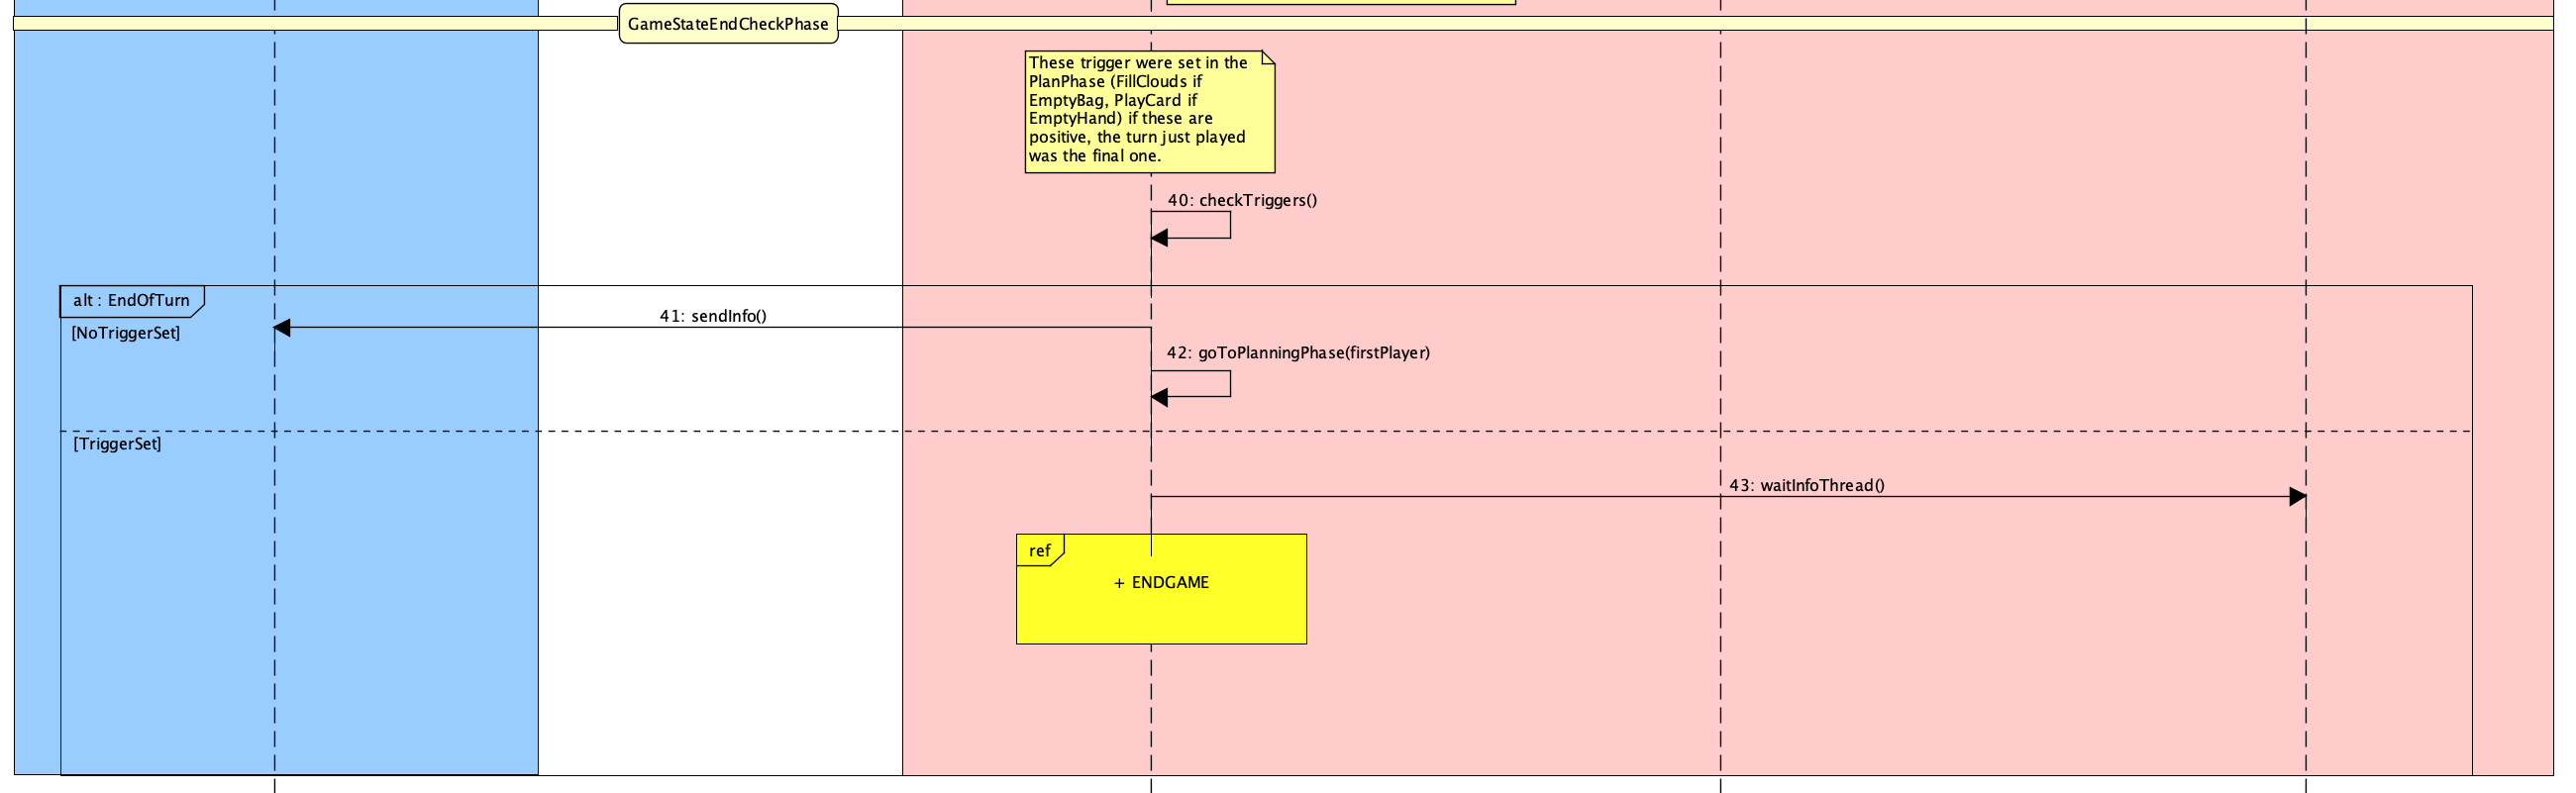
\includegraphics[width=\textwidth,height=\textheight,keepaspectratio]{Game_5}
				\end{center}
				
				First, the GameThread checks if any trigger (among EmptyBag or EmptyDeck) is set, if so the server enters the ``EndGame'', otherwise the server informs the players of the beginning of a new round with \emph{sendInfo()} and the GameThread returns back to the PlanningPhase.
				
			\begin{figure}[htp]
				\centering
				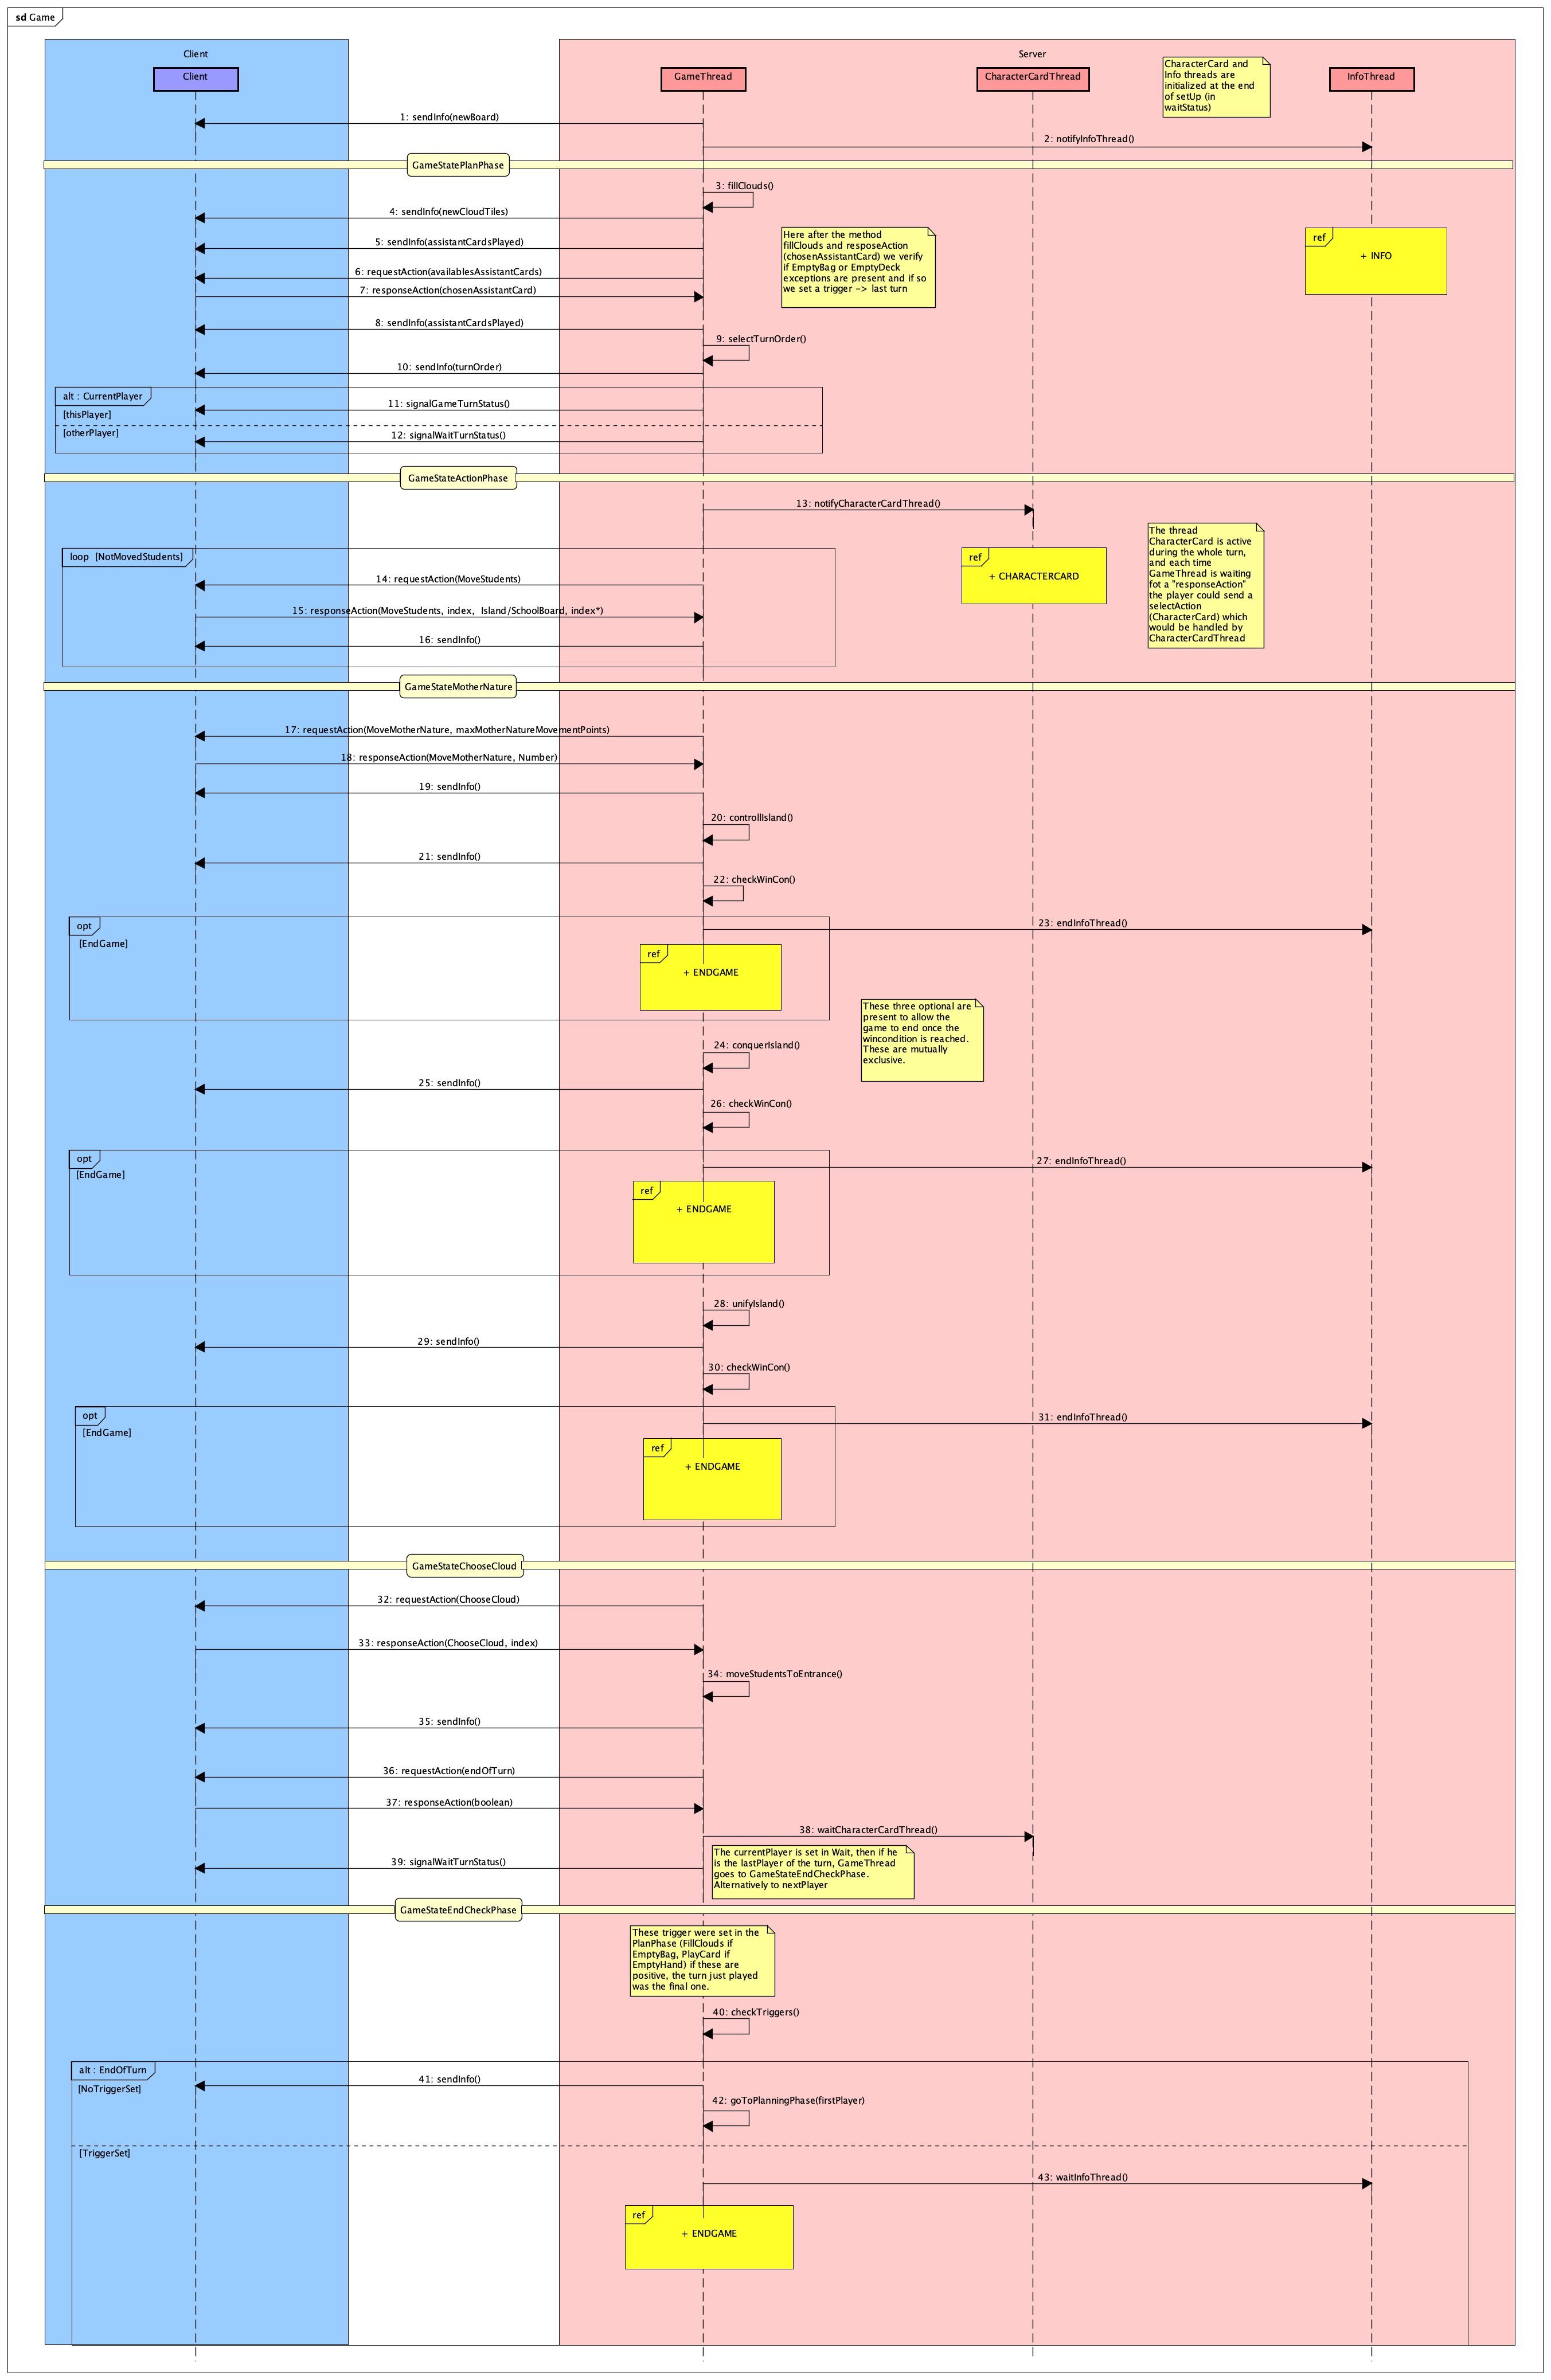
\includegraphics[width=\textwidth,height=\textheight,keepaspectratio]{Game}
			\end{figure}
			
			\newpage
			
		\subsection{Info}
			
			\begin{center}
				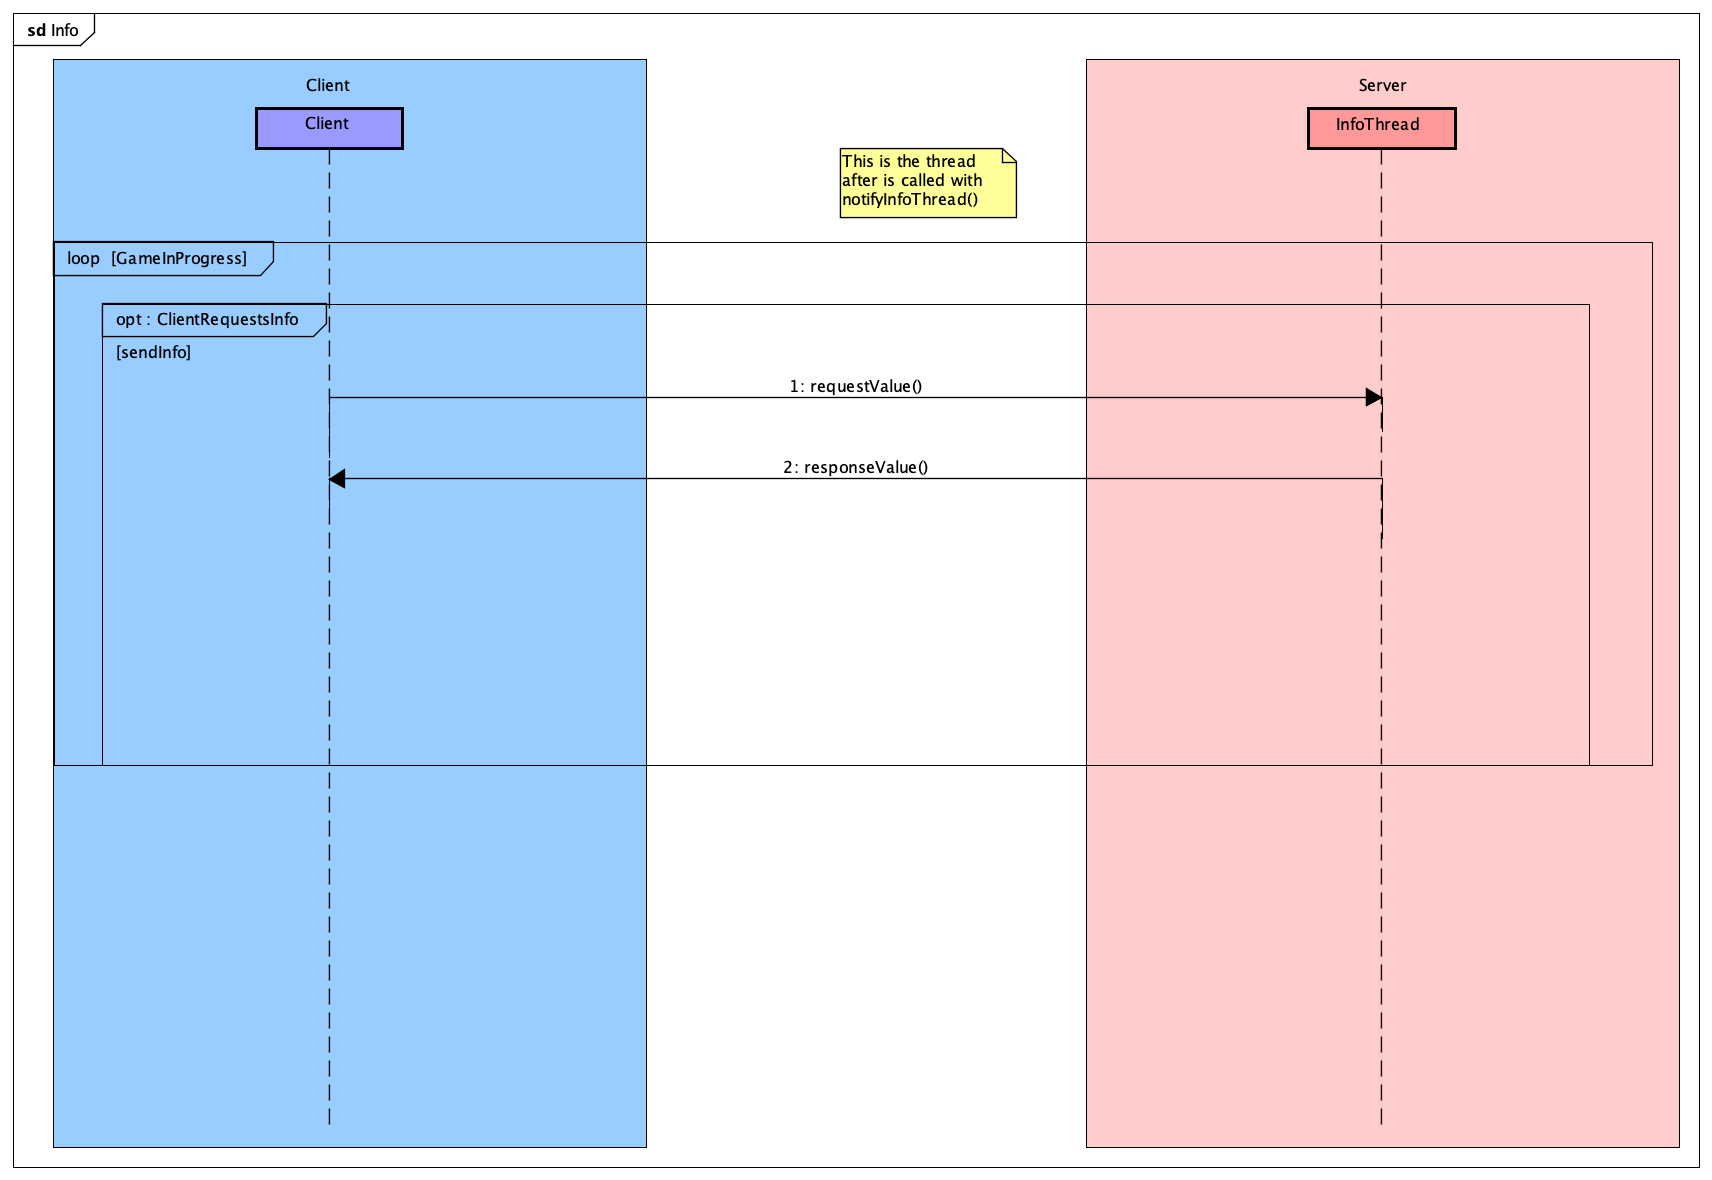
\includegraphics[width=\textwidth,height=\textheight,keepaspectratio]{img/Info}
			\end{center}
			
			During the Game, the players could ask for information about the Game's or the Model's status. These requests are handled concurrently with GameThread using a loop in the InfoThread. This thread is initialized once at the end of SetUpPhase and will be active until EndGame. When a \emph{requestValue()} is received by the InfoThread, it answers with a \emph{responseValue()} contaning the value of the field/attribute the player requested.
			
		\subsection{CharacterCard}
		
			\begin{center}
				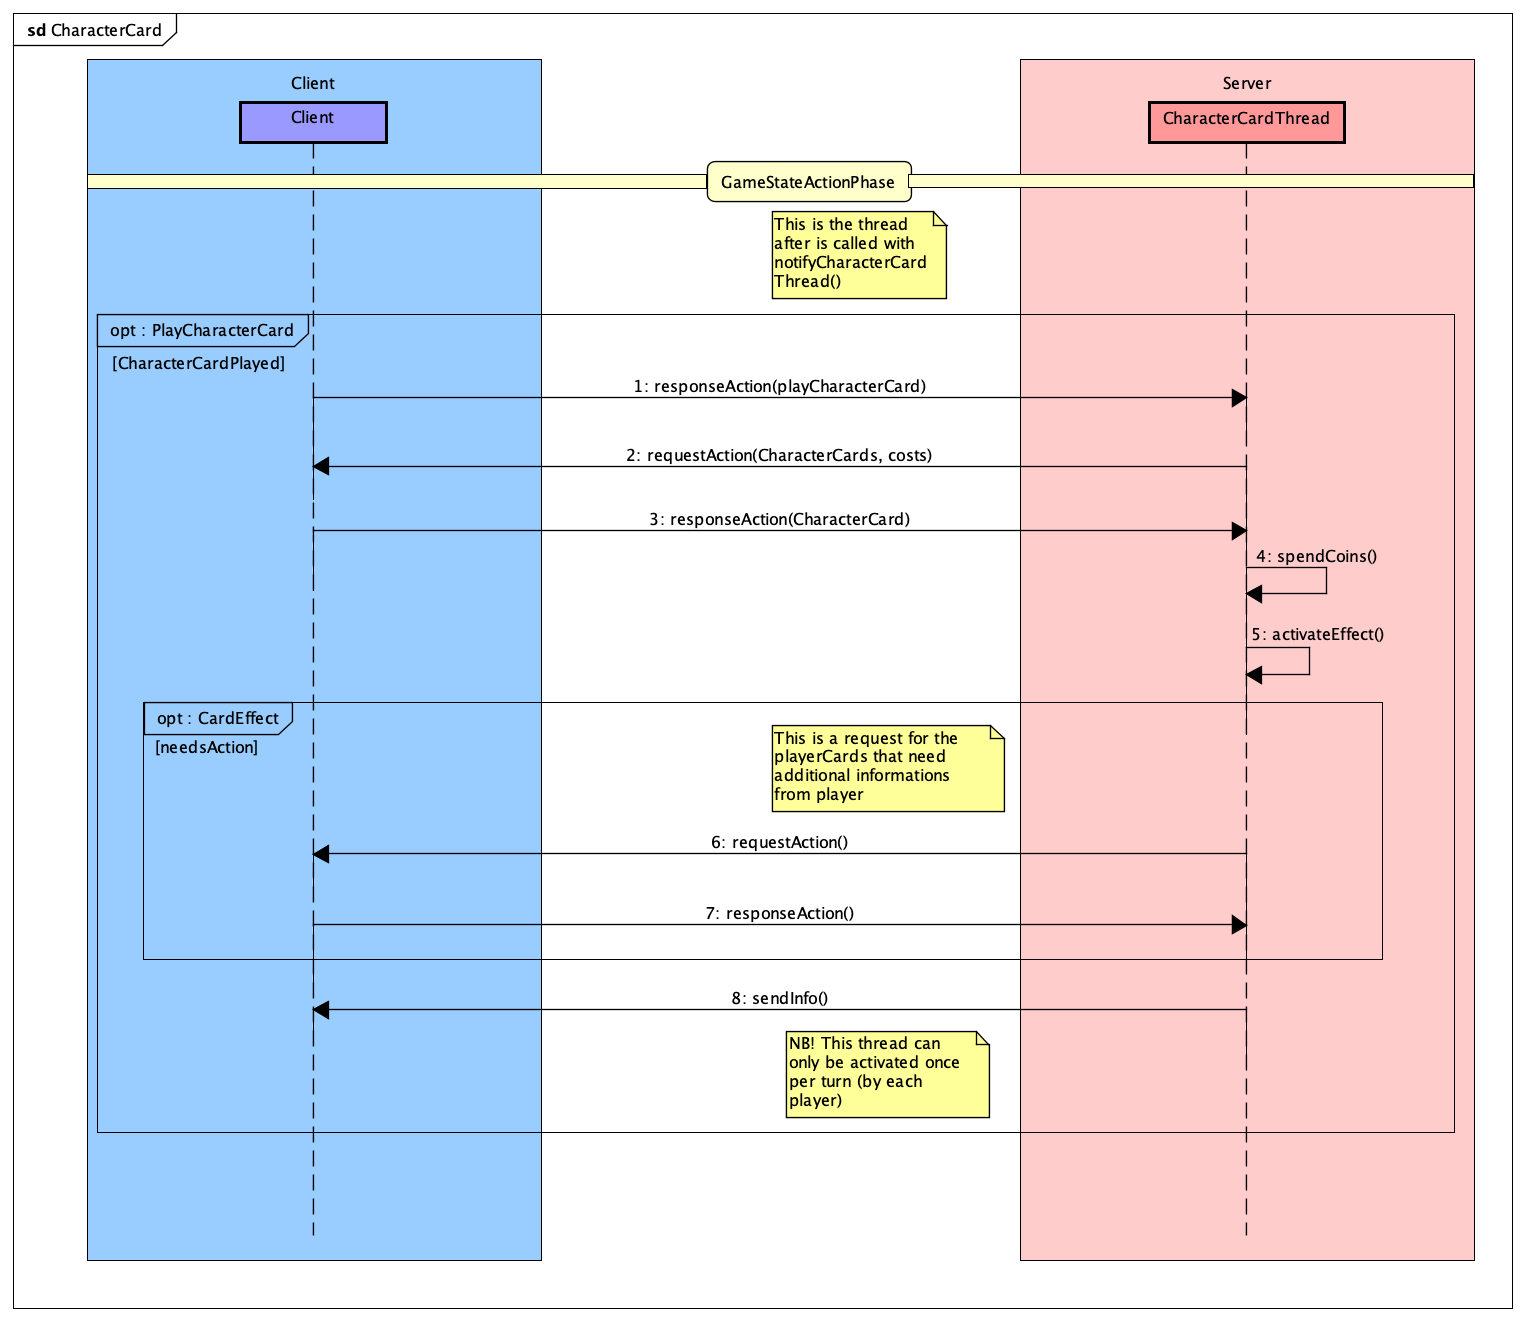
\includegraphics[width=\textwidth,height=\textheight,keepaspectratio]{CharacterCard}
			\end{center}
		
			During the Game, the players could ask to use one of the CharacterCards. These requests are handled concurrently with GameThread in the CharacterCardThread. This thread is initialized once at the end of the SetUpPhase and will be active until the EndOfTurn or the EndGame. When a \emph{responseAction(playCharacterCard)} is received by the CharacterCardThread, it answers with \emph{requestAction(CharacterCards, costs)} containing the available Cards to choose from and their respective costs. The client further responds with his choice in the message \emph{responseAction(CharacterCard)}. \\
			The server then proceeds to remove the coins from the player (if he has enough to pay the cost, else he sends an error message) and then activate the effect of the card. The card may need a further communication with the player (e.g.\ move a student counter or a no entry tile) so a server-client request-response is present as \emph{requestAction()} and \emph{responseAction()}. Once the effect of the card is activated the server informs the client with a \emph{sendInfo()}.
			
		\subsection{EndGame}
			
			\begin{center}
				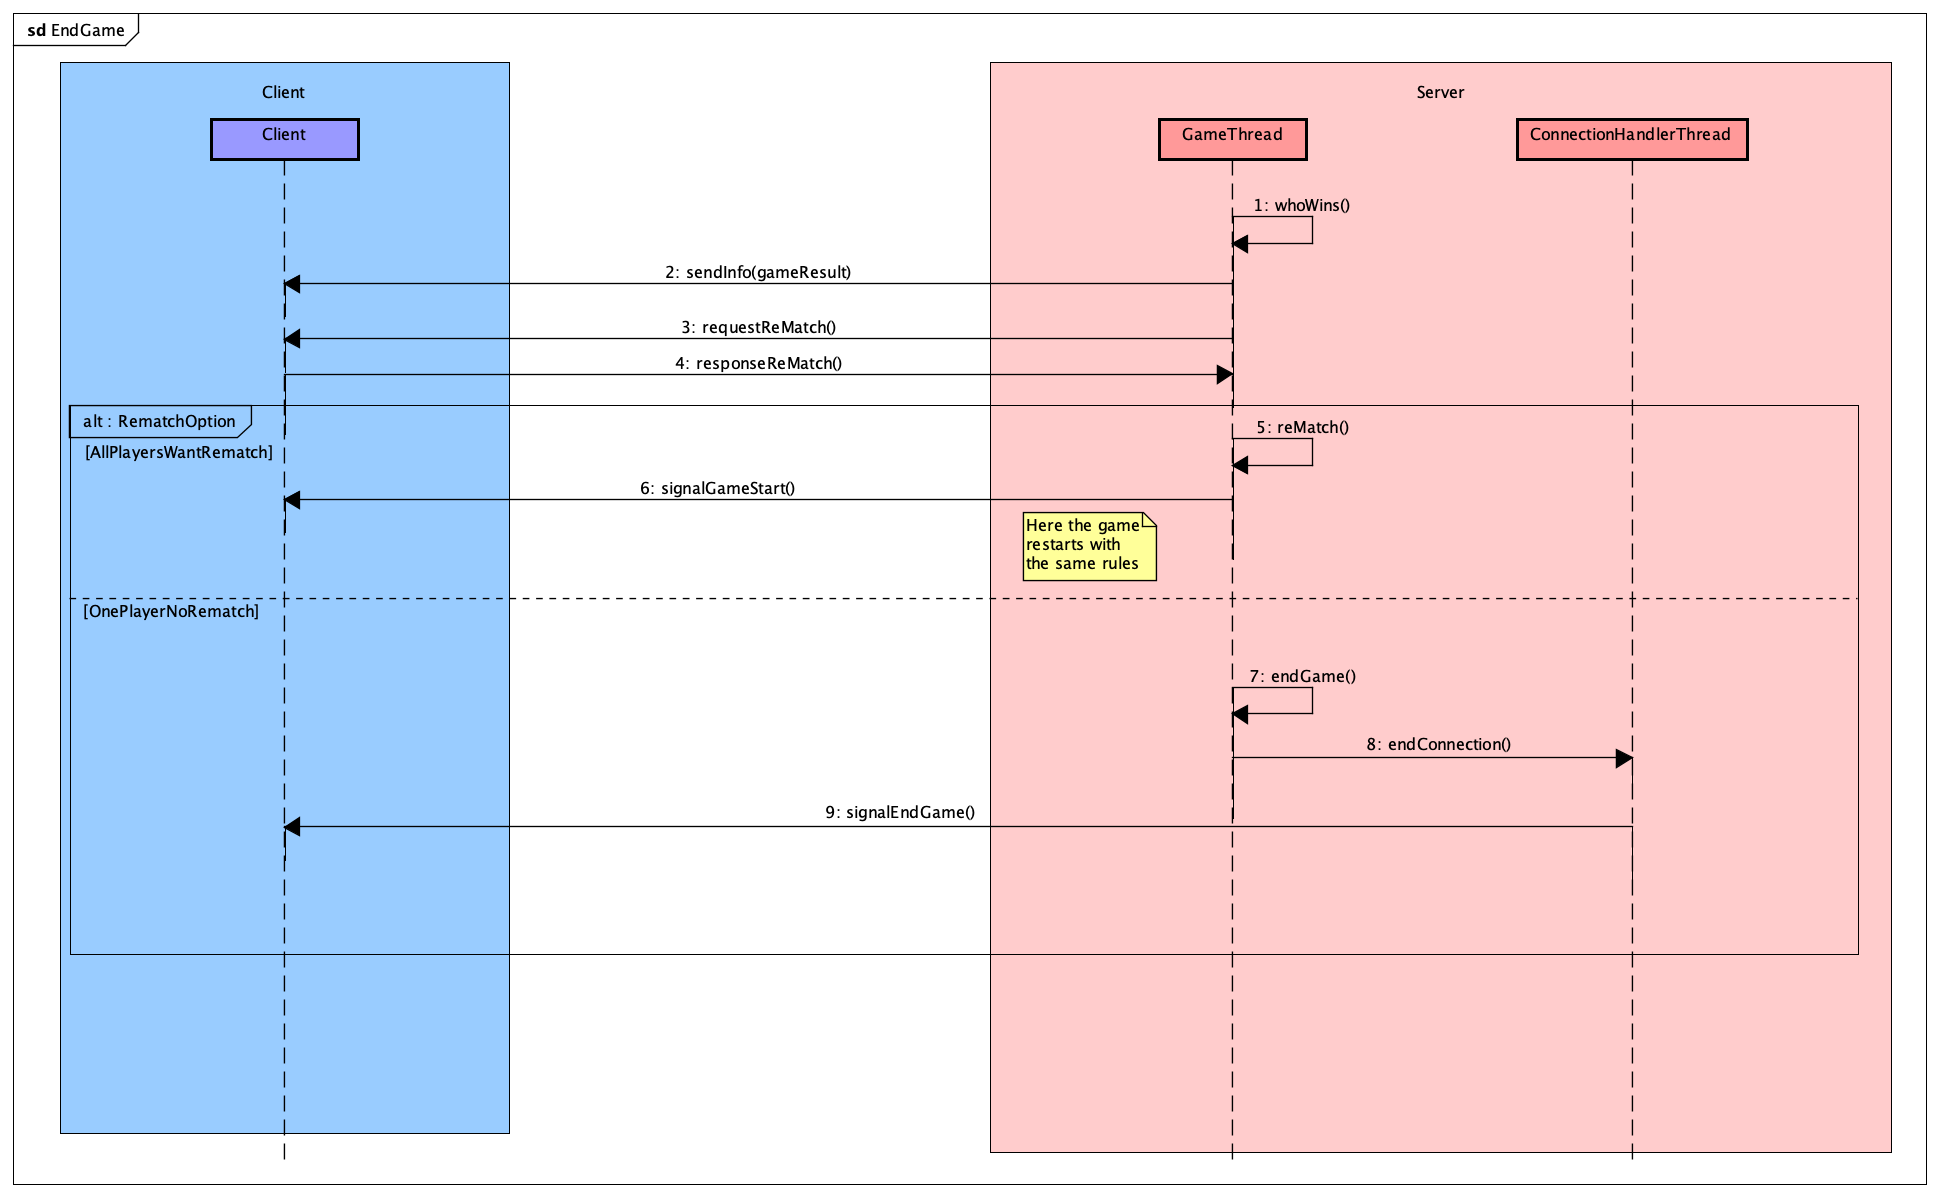
\includegraphics[width=\textwidth,height=\textheight,keepaspectratio]{EndGame}
			\end{center}	
			
			This is the final stage of the Game: the client will arrive to this stage being forwarded by other stages, once reached the winning condition or end-game condition (finishing student or assistantCard). First, the EndGame determines which player(s) won the game (or if a game is a draw), then sends the game result to all the partecipants via a \emph{sendInfo(gameResult)}. It sends also \emph{requestReMatch()} and waits for \emph{responseReMatch()}, where the player decides whether he wants to have another game, with the same players and the same rules, or not to do so.
			
			Thus, depending on the players’ responses to the server there could be two different scenarios:
			%
			\begin{itemize}
				%
				\item \textbf{AtLeastOnePlayerRefusedRematch}: the GameThread closes the current Game, then the ConnectionHandler closes the connection to all the players currently in the match.
				%
				\item \textbf{AllThePlayersAcceptedRematch}: the GameThread initializes a new GameBoard with the same rules of the previous game, then sends a \emph{signalGameStart()} to all the players, notifying them that a NewGame is starting.
				%
			\end{itemize}
			%
\end{document}